% Twoside implica che i capitoli inizino sempre con la prima pagina a sinistra, eventualmente lasciando una pagina vuota nel capitolo precedente. 
\documentclass[a4paper, twoside,openright]{report}

% Dimensione dei margini
\usepackage[a4paper,top=3cm,bottom=3cm,left=3cm,right=3cm]{geometry} 
% Dimensione del font
\usepackage[fontsize=12pt]{scrextend}
% Lingua del testo
\usepackage[english,italian]{babel}
% Lingua per la bibliografia
\usepackage[fixlanguage]{babelbib}
% Codifica del testo
\usepackage[utf8]{inputenc} 
% Encoding del testo
\usepackage[T1]{fontenc}
% Per modificare l'header delle pagine 
\usepackage{fancyhdr}               

\usepackage{float}

% Librerie matematiche
\usepackage{amssymb}
\usepackage{amsmath}
\usepackage{amsthm}         

% Uso delle immagini
\usepackage{graphicx}
% Uso dei colori
\usepackage[dvipsnames]{xcolor}         
% Uso dei listing per il codice
\usepackage{listings}          
% Per inserire gli hyperlinks tra i vari elementi del testo 
\usepackage{hyperref}     
% Diversi tipi di sottolineature
\usepackage[normalem]{ulem}

% -----------------------------------------------------------------

% Modifica lo stile dell'header
\pagestyle{fancy}
\fancyhf{}
\lhead{\rightmark}
\rhead{\textbf{\thepage}}
\fancyfoot{}
\setlength{\headheight}{16pt}

% Rimuove il numero di pagina all'inizio dei capitoli
\fancypagestyle{plain}{
  \fancyfoot{}
  \fancyhead{}
  \renewcommand{\headrulewidth}{0pt}
}

\definecolor{backcolour}{rgb}{0.90,0.95,0.92}

% Stile del codice
% \lstset{style=codeStyle}
\lstdefinestyle{codeStyle}{
    backgroundcolor=\color{backcolour},
    commentstyle=\color{teal},
    keywordstyle=\color{Magenta},
    numberstyle=\tiny\color{gray},
    stringstyle=\color{violet},
    basicstyle=\ttfamily\scriptsize,
    breakatwhitespace=false,     
    breaklines=true,                 
    captionpos=b,                    
    keepspaces=true,                 
    numbers=left,                    
    numbersep=5pt,                  
    showspaces=false,                
    showstringspaces=false,
    showtabs=false,
    tabsize=1
} \lstset{style=codeStyle}

% \lstset{style=longBlock}
\lstdefinestyle{longBlock}{
    commentstyle=\color{teal},
    keywordstyle=\color{Magenta},
    numberstyle=\tiny\color{gray},
    stringstyle=\color{violet},
    basicstyle=\ttfamily\scriptsize,
    breakatwhitespace=false,         
    breaklines=true,                 
    captionpos=b,                    
    keepspaces=true,                 
    numbers=left,                    
    numbersep=5pt,                  
    showspaces=false,                
    showstringspaces=false,
    showtabs=false,                  
    tabsize=2
} \lstset{style=codeStyle}

% Togliendo il commento al comando che segue, si inseriscono nella bibliografia anche le fonti presenti in Bibliography.bib ma non citati direttamente con il comando \cite
\nocite{*}

% Margini prima e dopo blocchi di codice, per avere più distanza
\lstset{aboveskip=20pt,belowskip=20pt}

% Modifica dello stile dei riferimenti
\hypersetup{
    colorlinks,
    linkcolor=black,
    citecolor=black
}

% Aggiunti definizioni, teoremi, linea e listing
\newtheorem{definition}{Definizione}[section]
\newtheorem{theorem}{Teorema}[section]
\providecommand*\definitionautorefname{Definizione}
\providecommand*\theoremautorefname{Teorema}
\providecommand*{\listingautorefname}{Listing}
\providecommand*\lstnumberautorefname{Linea}

\raggedbottom



% -----------------------------------------------------------------
\begin{document}
\begin{titlepage}
\begin{figure}[!htb]
    \centering
\end{figure}
\vspace{30mm}
\begin{center}
    \LARGE{POLITECNICO DI TORINO}
    \vspace{5mm}
\end{center}

\vspace{15mm}
\begin{center}        
    {\LARGE{\bf Fundamentals of Information Systems Security}}
\end{center}
\vspace{30mm}

\hfill
\begin{center}

\large{Student:}
{\normalsize\vspace{3mm} \bf\\ \large{Gianmarco Michelini}}
\end{center}


\vspace{30mm}
\hrulefill
\\\centering{\large{Academic Year 2024/2025}}

\end{titlepage}
\let\cleardoublepage\clearpage

\tableofcontents
\listoffigures

\chapter{Cryptographic Techniques}
\cite{02_basic_crypto}.
Cryptography is the practice of securing communication and data by transforming it into a format that is unreadable to unauthorized users. It uses mathematical algorithms to encrypt (scramble) and decrypt (unscramble) information, ensuring confidentiality, integrity, authentication, and non-repudiation in digital communications.

The message in its original, unencrypted form is called plaintext (or cleartext), referred to as P. On the other hand, the message after being encrypted is called ciphertext, referred to as C. 

\section{Symmetric Cryptography}
\begin{center}
    Only one key, shared between the sender and the receiver, is used for both encryption and decryption. 
\end{center}
Pros and cons:
\begin{itemize}
    \item Key distribution problems (lots of keys for a complete pairwise private communication).
    \item Key management problems.
    \item Faster than asymmetric cryptography.
    \item Main utility: data confidentiality.
\end{itemize}



\begin{multicols}{2}

    \textbf{Encrypt Equation}
\begin{equation*}
    \begin{aligned}
        C &= \text{enc}(K, P) \\
          &= \{ P \}_K
    \end{aligned}
\end{equation*}

\hfill

\textbf{Decrypt Equation}
\begin{equation*}
    \begin{aligned}
        P &= \text{dec}(K, C) \\
          &= \text{enc}^{-1}(K, C)
    \end{aligned}
\end{equation*}
    \columnbreak
    
    \begin{figure}[H]
        \centering
        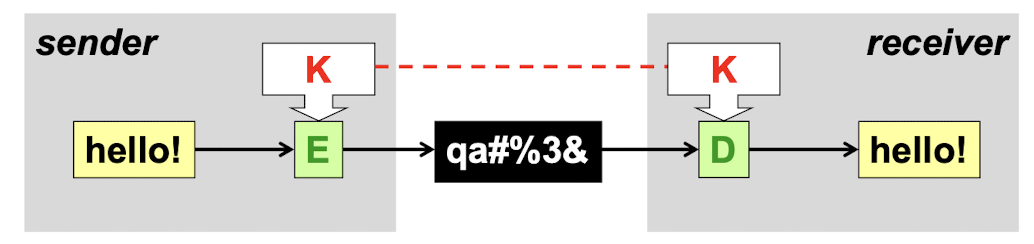
\includegraphics[width=\linewidth]{Images/Cryptography/symmCrypto.png}
        \caption{Example of symmetric encryption}
    \end{figure}
\end{multicols}

\clearpage

\subsection{Symmetric Block Encryption Algorithms}
Block encryption refers to ciphers that process fixed-size blocks of data (e.g., 128 bits for AES) at a time.

\begin{figure}[H]
    \centering
    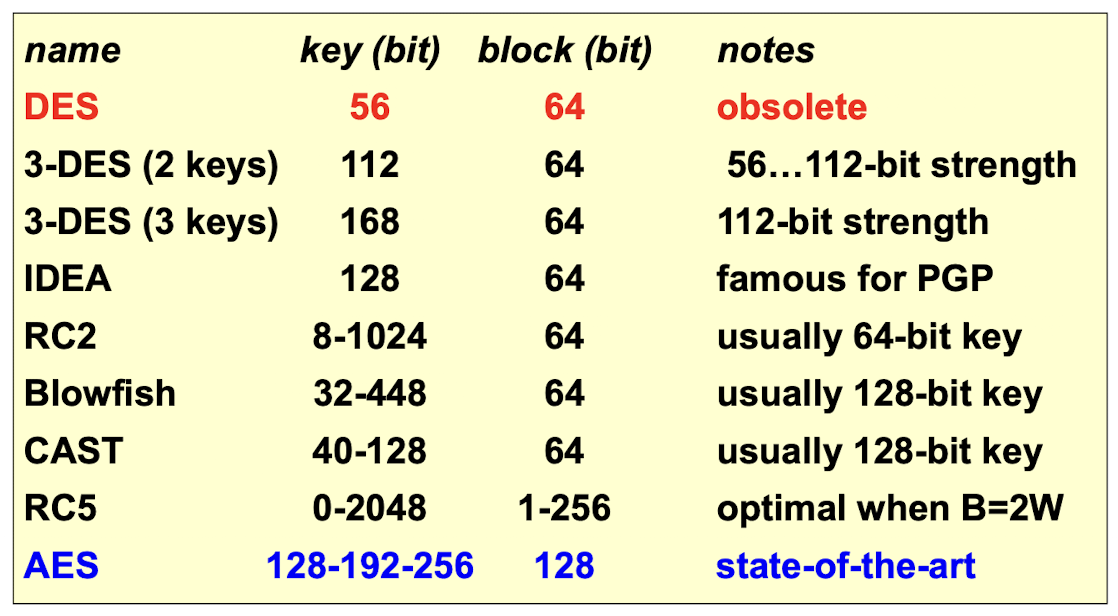
\includegraphics[width=0.5\linewidth]{Images/Cryptography/blockSymm.png}
    \caption{Famous Symmetric Block Encryption Algorithms}
\end{figure}


\subsubsection{Data Encryption Standard}
\begin{center}
    (DES - Obsolete because of short key length)

    56-bit key, 64-bit block.
\end{center}
Is a symmetric-key block cipher that was widely used for data encryption in the past. It was developed in the 1970s by IBM.

The key features are:
\begin{itemize}
    \item Block cipher: DES operates on 64-bit (8 bytes) blocks of data, meaning it encrypts 64 bits of plaintext at a time.
    \item Key length: DES uses a 56-bit (7 bytes) key.
    \item Efficient in hardware: Requires only XOR, shift and permutation.
\end{itemize}

\subsubsection{Triple DES}
\begin{center}
    (3DES or TDES)

    112 or 168-bit key, 64-bit block, EDE mode for backward compatibility.
\end{center}

Is a symmetric-key block cipher that was developed to enhance the security of the original DES.

The key features are:
\begin{itemize}
    \item Block cipher: like DES (8 bytes).
    \item Key Length: 3DES can use either:
    \begin{itemize}
        \item \textbf{Two keys} (2-key 3DES): The first and third keys are the same, resulting in a 112-bit effective key length.
        \item \textbf{Three keys} (3-key 3DES): All three keys are distinct, resulting in a 168-bit effective key length.
    \end{itemize}
    \item Triple encryption: 3DES applies the DES algorithm three times to each data block, using either two (2-key 3DES) or three (3-key 3DES) distinct keys.
    \item Is typically applied in the Encrypt-Decrypt-Encrypt (EDE) mode to achieve compatibility with DES when.
\end{itemize}

\subsubsection*{EDE Mode}
In this mode, the data is first encrypted using the first key, then decrypted using the second key, and finally encrypted again using the third key (if a third key is present). This sequence of operations helps mitigate the vulnerabilities of DES by applying encryption multiple times.

\begin{tcolorbox}[colback=blue!10!white, colframe=blue!50!white, title=Meet-in-the-Middle attack]
    Double application of encryption algorithms is subject to a known plaintext attack named meet-in-the-middle, which allows decrypting data with at most $2^{N+1}$ attempts (the key is N-bit long).
    For more details, refer to Appendix A.
\end{tcolorbox}

\subsubsection{Advanced Encryption Standard}
\begin{center}
    AES.
\end{center}
In order to replace DES.

\begin{itemize}
    \item Symmetric block cipher.
    \item Developed by Joan Daemen and Vincent Rijmen.
    \item Key features:
    \begin{itemize}
        \item Block size: 128 bits.
        \item Key length: 128, 192, or 256 bits.
    \end{itemize}
\end{itemize}

\begin{tcolorbox}[colback=blue!10!white, colframe=blue!50!white]
Ciphers are like wine: the older, the better.
\end{tcolorbox}


\subsection{Application Modes for Block Algorithms}
Block ciphers split the data (plaintext) into fixed-size blocks.

We should answer a question:
\begin{tcolorbox}[colframe=lightblue]
    \begin{center}
        \textit{Is the size of the data to encrypt smaller or larger than \newline the algorithm's block size?}
    \end{center}
\end{tcolorbox}
    

If the answer is:
\begin{itemize}
    \item Size of the data to encrypt > algorithm's block size: Use Electronic Code Book (ECB) or Cipher Block Chaining (CBC).
    \item Otherwise (size of the encrypted data not a multiple of the block size): Padding, Cipher FeedBack (CFB), Output FeedBack (OFB) or Counter Mode (CTR).
\end{itemize}

\subsubsection{Electronic Code Book}
\begin{center}
    (ECB)
\end{center}

Simple mode of operation for block ciphers. In this mode, the plaintext is divided into fixed-size blocks, and each block is encrypted independently using the same key.

\begin{multicols}{2}
    \begin{equation*}
        \boxed{C_i = enc \ (K, P_i)}
    \end{equation*}
    \begin{figure}[H]
        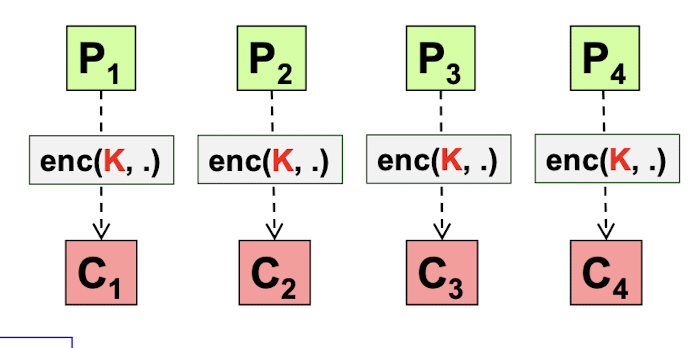
\includegraphics[width=\linewidth]{Images/Cryptography/ECBEncrypt.png}
        \caption{ECB encrypting.}
    \end{figure}
    \columnbreak
    \begin{equation*}
        \boxed{P_j = \text{enc}^{-1}(K, C_j)}
    \end{equation*}
    \begin{figure}[H]
        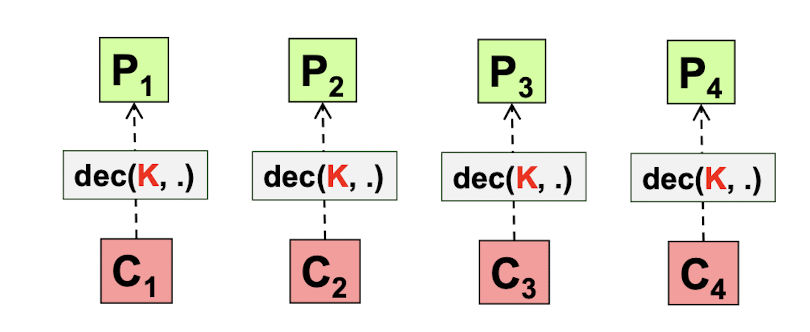
\includegraphics[width=\linewidth]{Images/Cryptography/ECBDecrypt.png}
        \caption{ECB decrypting.}
    \end{figure}
\end{multicols}

Key features:
\begin{itemize}
    \item Should not be used for long messages because swapping two blocks of ciphertext goes undetected.
    \item Each block is encrypted separately with the block cipher using the same key.
    \item The encrypted blocks are concatenated to produce the ciphertext.
    \item Identical plaintext blocks produce identical ciphertext blocks, which can lead to patterns in the ciphertext that may be exploited in cryptanalysis.
    \item If there is an error in one ciphertext block  $C_j$ , only the corresponding plaintext block  $P_j$  will be affected during decryption.
\end{itemize}

\clearpage
\subsubsection{Cipher Block Chaining}

\begin{center}
    (CBC)
\end{center}
Mode of operation for block ciphers that provides better security than Electronic Codebook (ECB). It involves chaining the encryption of each block with the previous block's ciphertext, which helps obscure patterns in the ciphertext.


\begin{multicols}{2}
    \begin{equation*}
        \boxed{C_i = enc \ (K, P_i \oplus C_{i-1})}
    \end{equation*}
    \begin{figure}[H]
        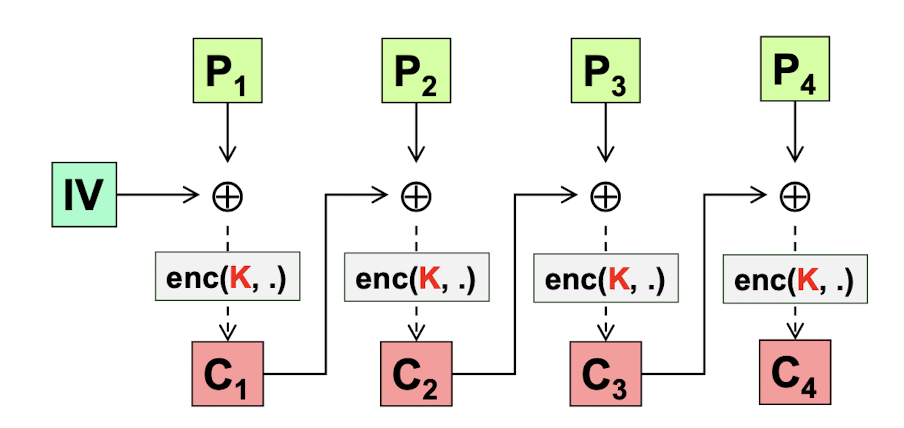
\includegraphics[width=\linewidth]{Images/Cryptography/CBCEncrypt.png}
        \caption{ECB encrypting.}
    \end{figure}
    \columnbreak
    \begin{equation*}
        \boxed{P_j = \text{enc}^{-1}(K, C_j) \oplus C_{j-1}}
    \end{equation*}
    \begin{figure}[H]
        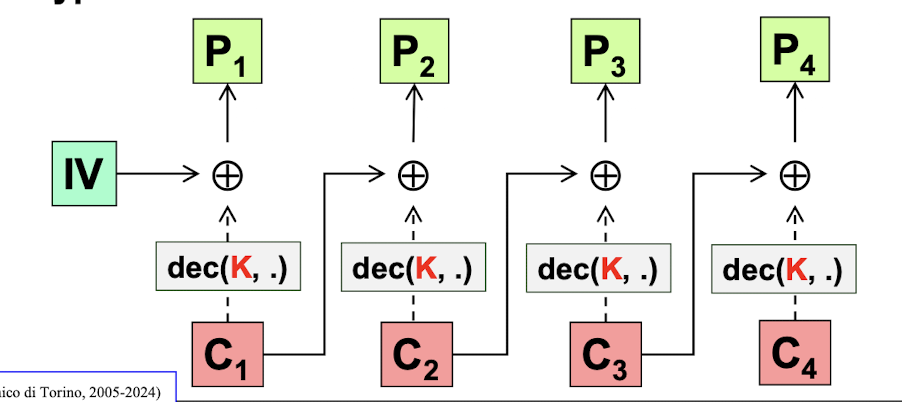
\includegraphics[width=\linewidth]{Images/Cryptography/CBCDecrypt.png}
        \caption{ECB decrypting.}
    \end{figure}
\end{multicols}

Key features:
\begin{itemize}
    \item Requires an Initialization Vector (IV=$C_0$).
    \item XOR between ciphertexts and plaintexts.
    \item If there is an error in a ciphertext block $C_j$ it will affect the decryption of two blocks of plaintext:
    \begin{itemize}
        \item The current block $P_j$ will be corrupted because the error will be decrypted into some incorrect plaintext. 
        \item The next block  $P_{j+1}$  will also be corrupted because the error will propagate into the XOR operation with the next ciphertext block  $C_{j+1}$.
    \end{itemize} 
\end{itemize}

\clearpage

\subsubsection{Padding}
\begin{center}
    Scopes: aligning, filling. Always add data to a block.
\end{center}

Padding is used in block cipher encryption schemes to handle plaintext that is not an exact multiple of the block size. Since block ciphers operate on fixed-size blocks, any plaintext that does not fit into the required block size needs to be padded.
\begin{figure}[H]
    \centering
    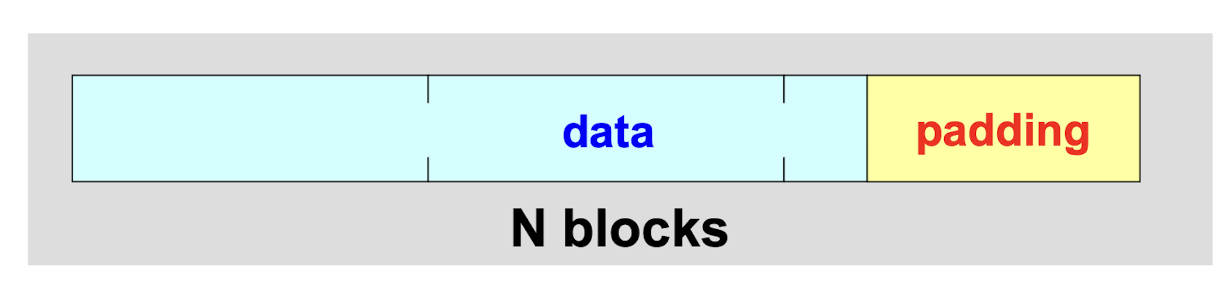
\includegraphics[width=0.5\linewidth]{Images/Cryptography/padding.png}
    \caption{Padding Mode}
    
\end{figure}

\subsubsection*{Padding Techniques}
\begin{itemize}
    \item Original DES Padding: bit pattern that started with a 1 bit, followed by many 0 bits.
    \item One byte with value 128 (0x80) followed by null bytes.
    \item Last byte indicates padding length.
    \item Padding with explicit length:
    \begin{itemize}
        \item Null bytes, with the last byte indicating the padding length.
        \item Only null bytes. \textcolor{Blue}{Schneier}
        \item Bytes with value equal to Length. \textcolor{Blue}{SSL/TLS}
        \item Random bytes. \textcolor{Blue}{SSH2}
        \item Sequential numbers starting from 0x01. \textcolor{Blue}{IPSec/ESP}
        \item Each byte is the $Length-1$.
    \end{itemize}
\end{itemize}

\subsubsection*{Some Keynotes}
\begin{itemize}
    \item Minimal integrity control: If the key is incorrect or data were manipulated, the padding bytes will become incoherent.
    \item Typically applied to large data, on the last fragment.
    \item If the data length D is less than the block size B, ad-hoc techniques like CFB, OFB, or CTR are preferred instead of padding.
    \item \textbf{Even if the plaintext is an exact multiple of the block size, padding is still required to avoid errors in the interpretation of the last block.}
\end{itemize}

\subsubsection{Cipher Text Stealing}
\begin{center}
    (CTS)
\end{center}
Allows the use of block algorithms without adding new data to a block (e.g. padding).

Process (using CTS-ECB):
\begin{itemize}
    \item Uses CBC until the last block of the plaintext.
    \item The second-to-last block is encrypted and divided into two parts (head + tail, the tail is the same size as the gap of the plaintext $n$).
    \item The last (partial) block is filled with the tail from the second-to-last block.
    \item The "new" last block (old last block + tail, now "full") is encrypted.
    \item After encryption, the positions of the last and second-to-last block (only the "head") are swapped.
\end{itemize}
This method is particularly useful when the size of the data cannot be increased after encryption, such as in storage encryption.

\textbf{However, the computation time increases slightly}.

\begin{multicols}{2}

    \begin{figure}[H]
        \centering
        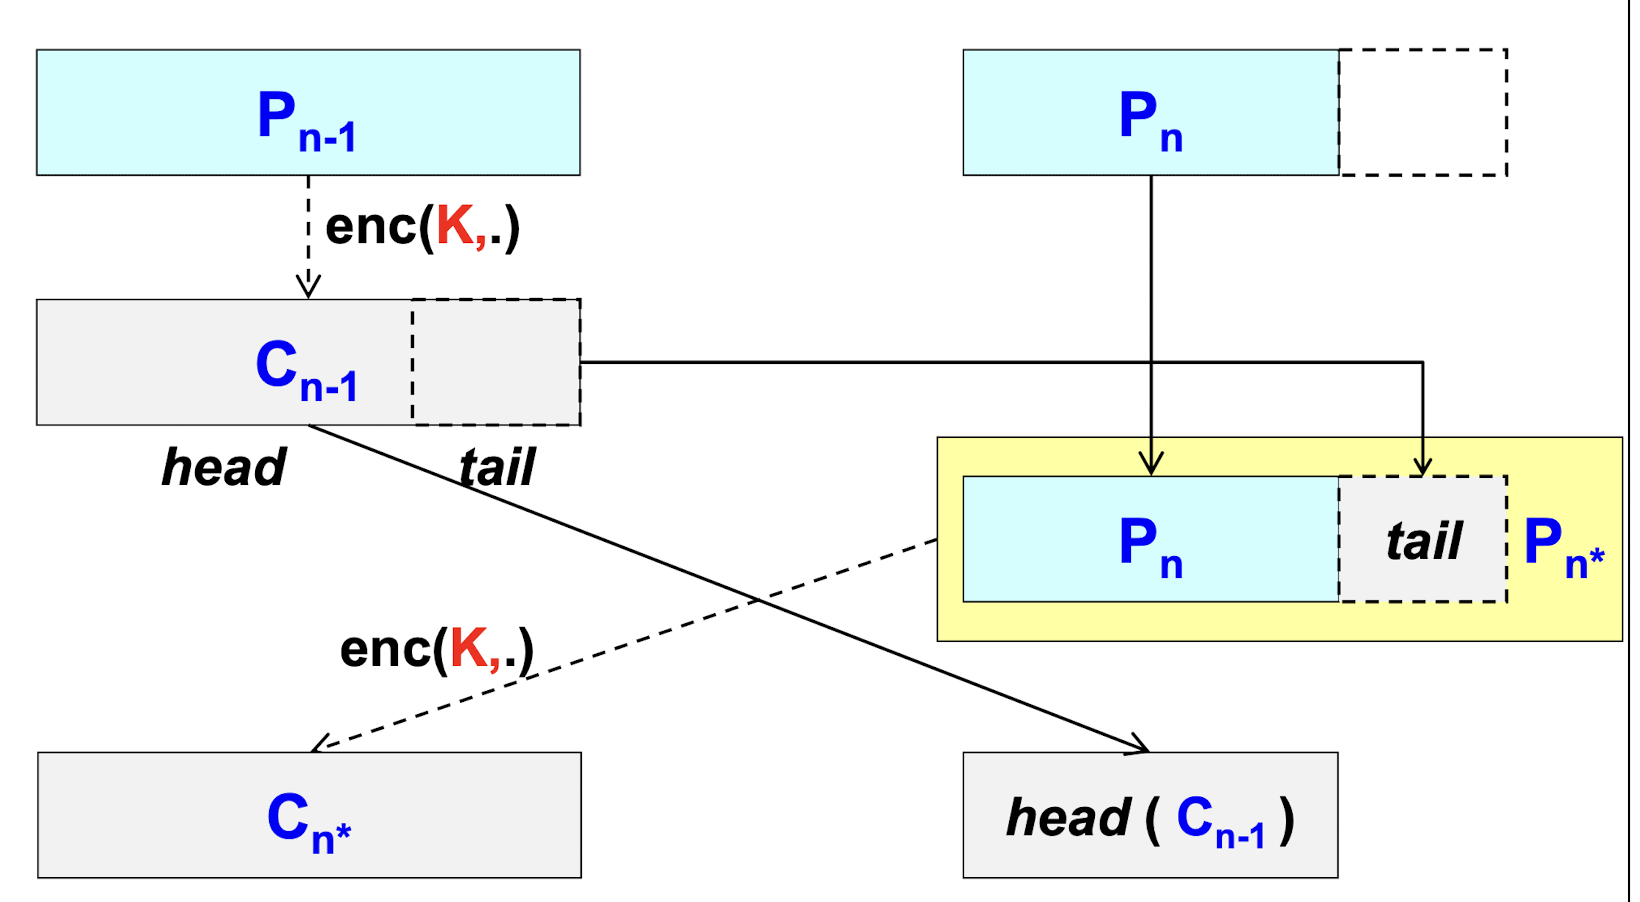
\includegraphics[width=\linewidth]{Images/Cryptography/CTS_ECB.png}
        \caption{CTS with ECB}
    \end{figure}

    \columnbreak

    \begin{figure}[H]
        \centering
        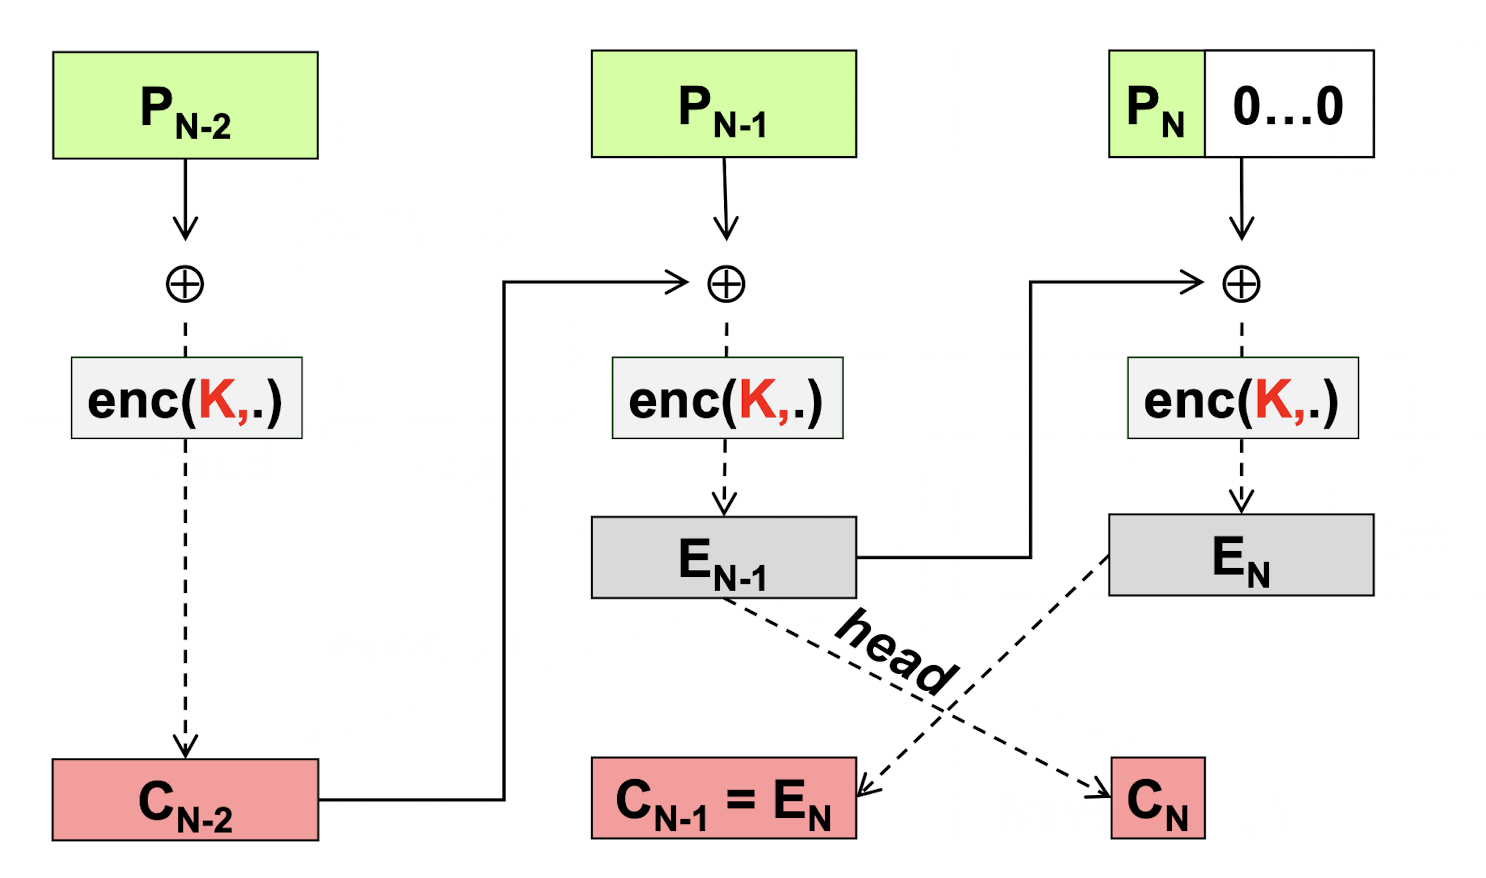
\includegraphics[width=\linewidth]{Images/Cryptography/CTS_CBC.png}
        \caption{CTS with CBC}
    \end{figure}
    
\end{multicols}

\clearpage 
\subsubsection{Counter Mode}
\begin{center}
    (CTR)
\end{center}
Requires a \textbf{nonce} and a \textbf{counter}, combined to generate the input block.

Key features:
\begin{itemize}
    \item The nonce is a random number that should never be reused with the same data.
    \item The counter is a value that is incremented for each block.
    \item The input block is encrypted using the block cipher, generating a fixed-size encrypted "unique" block.
    \item The leftmost group\footnote{Meaning the first N bits, based on the required $plaintext\_size$.} is extrapolated from the block and are XORed with the corresponding $P_i$ group, which in turn generates the corresponding $C_i$ group.
    \item The same process is repeated for each successive plaintext group, with the counter incremented each time.
\end{itemize}

\begin{figure}[H]
    \centering
    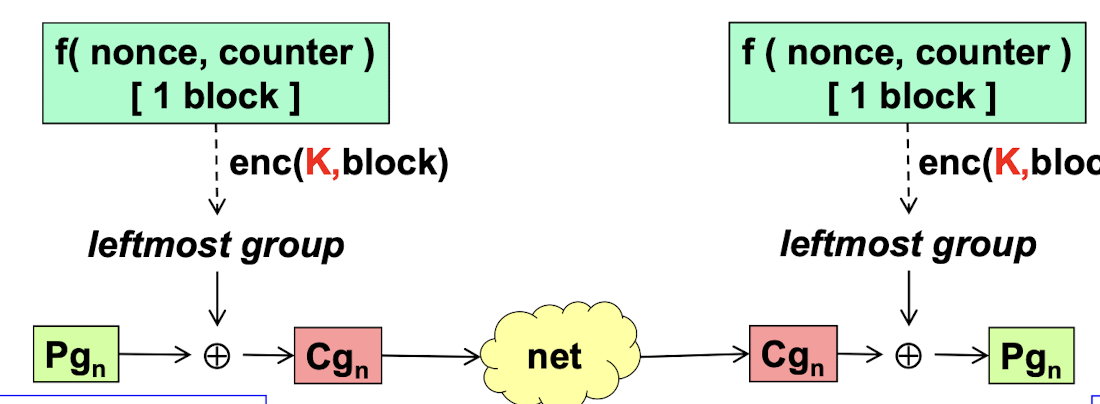
\includegraphics[width=0.6\linewidth]{Images/Cryptography/CTR_ENC.png}
    \caption{CTR Mode}
\end{figure}


\subsection{Symmetric Stream Encryption Algorithms}
\begin{center}
    Byte-by-byte(or bit-by-bit) encryption.

    No fixed-size block boundaries.
\end{center}
Stream encryption refers to ciphers that process data one bit or byte at a time.





\begin{multicols}{2}


    Main features:
    \begin{itemize}
        \item Ideal algorithm: One-Time Pad (OTP), requires a key as long as the plaintext to protect.
        \item Real algorithms: Use pseudo-random number generators (PRNGs) to generate a key stream, \textbf{synchronized} between sender and receiver.
        \item Modern: Salsa20, ChaCha20.
    \end{itemize}
\columnbreak

\begin{figure}[H]
    \centering
    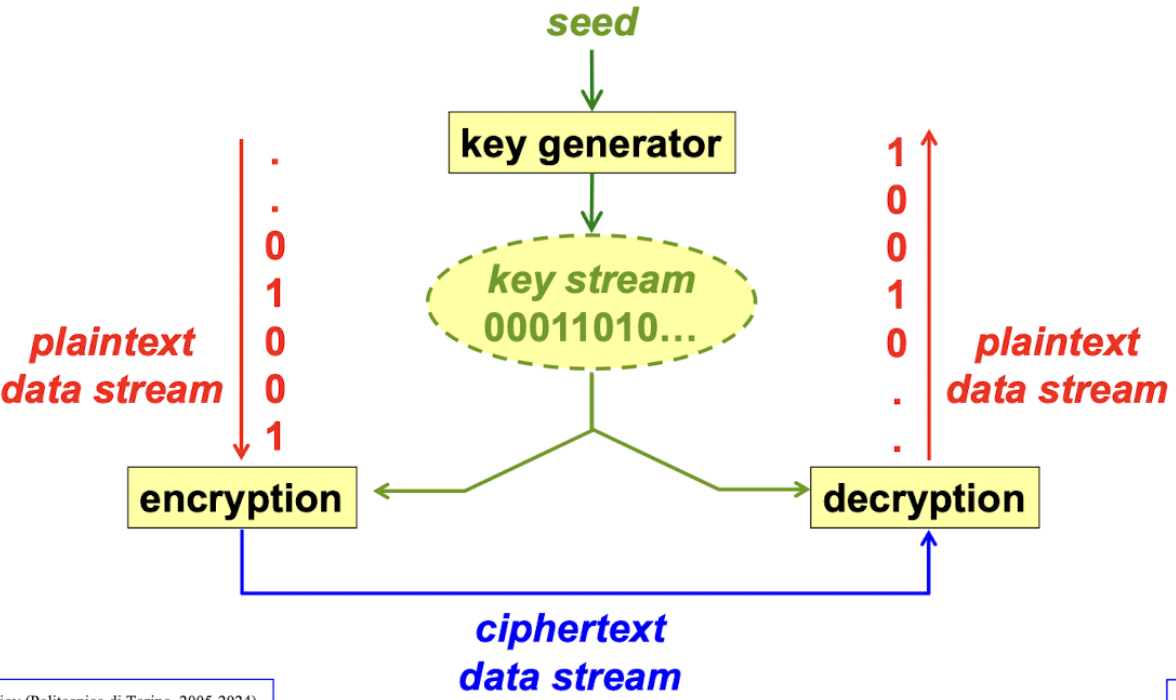
\includegraphics[width=\linewidth]{Images/Cryptography/Stream_Cipher.png}
    \caption{Stream (real) algorithm process.}
\end{figure}
\end{multicols}

\subsubsection{Salsa20}
\begin{center}
    128 or 256-bit Key.
\end{center}

Key features:
\begin{itemize}
    \item 128 or 256-bit Key.
    \item Base operation: 32-bit ARX (Addition, Rotation, XOR).
    \item Base function: f(Key \textcolor{Blue}{(256 bits)}, Nonce \textcolor{Blue}{ 64}, Counter \textcolor{Blue}{ 64}) = 512-bit keystream block.
    \item Can process 64-byte blocks of data.
    \item Allows random access decryption: Since each block is encrypted independently, it is possible to decrypt any block at random without needing to decrypt the preceding blocks.
    \item Can securely encrypt $64B \cdot 2^{64}$ blocks of data with a single key and nonce pair.
\end{itemize}
\subsubsection{ChaCha20}
An improved version of Salsa20, designed to provide better security and performance. So inherit the same features as Salsa20.
\begin{center}
    ChaCha20 and Poly1305 for IETF protocols.
\end{center}
Slightly modifications to the original specification:
\begin{itemize}
    \item 96 bit nonce (from 64).
    \item 32 bit lock counter (from 64).
    \item Hence, a limit of $2^{32} \cdot \ 64$ byte blocks. That corresponds to 256 GB of data (amount of data that can be encrypted with a single key and nonce pair) with a 64-byte block size.
\end{itemize}

\section{Comparison of Symmetric Ciphers}



\begin{multicols}{2}

    Stream algorithms:
    \begin{itemize}
        \item Works on variable length data stream (faster computation).
        \item Need a synchronized key stream (synch problems between the parties).
        \item Reliable pseudo random number generator (PRNG).
    \end{itemize} 
\columnbreak

Block algorithms:
\begin{itemize}
    \item Split data into fixed-size blocks (slower computation).
    \item Attacks based on the mode of operation (e.g. ECB).
    \item May be used padding, so additional data to the message.
\end{itemize}
\end{multicols}

\section{Kerchoffs' Principle}
\begin{quotation}
    If the keys are kept secret, managed securely (well-designed algorithm and executed by a trusted party), and are long enough, the system remains secure even if the encryption and decryption algorithms are publicly known. 
\end{quotation}
    This is because, without access to the keys, an attacker cannot decrypt the data. In fact, making the algorithms public allows the cryptographic community to rigorously test and analyze them for potential weaknesses, improving the overall security of the system.


\subsection*{Attempts to Perform an Exhaustive Search}
Assuming that Kerchoffs' Principle is respected. Considering a key of length N bits.

\dots The only possible attack is the brute force (exhaustive search) attack, which requires $2^N$ attempts.

\[
    \boxed{T \propto 2^N}
\]

\subsection{Key Distribution for Symmetric Cryptography}
\raggedcolumns
\begin{multicols}{2}

\noindent For a complete pairwise private communication between N parties, we need:
\begin{center}
    $\boxed{\displaystyle\frac{N \cdot (N-1)}{2}}$ keys.
\end{center}

\columnbreak

    \begin{figure}[H]
        \centering
        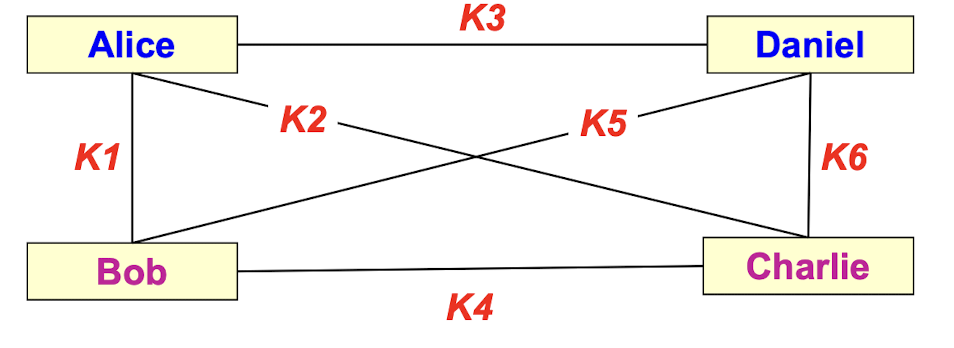
\includegraphics[width=\linewidth]{Images/Cryptography/key_dist_symm.png}
        \caption{Key Distribution}
    \end{figure}
\end{multicols}


Distribution Methods:
\begin{itemize}
    \item Out-Of-Band (OOB): Keys are exchanged using a separate, secure communication channel (e.g., in person or using a different secure network).
    \item Key exchange algorithms.
\end{itemize}


\section{Minimum Acceptable Key Length (2025)}
\begin{itemize}
    \item 128 bits for symmetric algorithms.
    \item 2048 bits for asymmetric algorithms.
    \item 256 bits for cryptographic hash functions.
\end{itemize}
\begin{figure}[H]
    \centering
    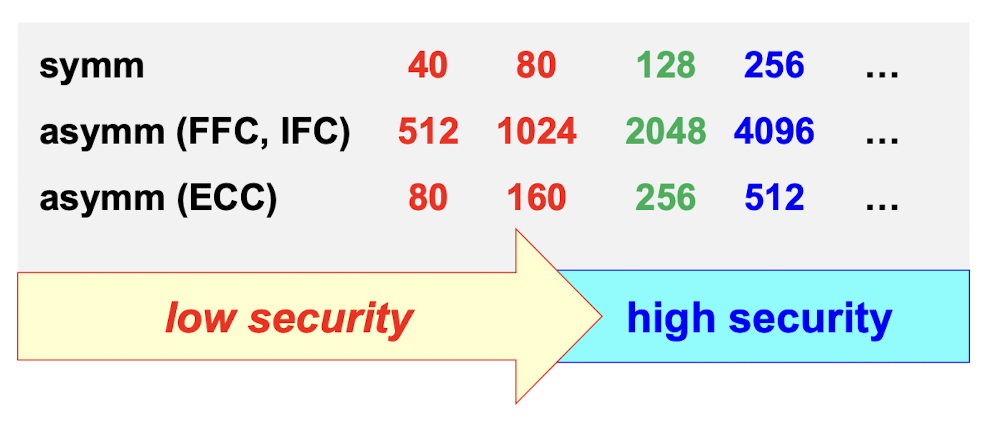
\includegraphics[width=0.5\linewidth]{Images/Cryptography/crypto_key_lens.png}
    \caption{Key length of cryptographic algorithms}
\end{figure}

\section{Asymmetric Cryptography}
\begin{center}
    Used for confidentiality without shared secrets or digital signatures.
\end{center}
AKA public-key cryptography.
Each person has a different key pair (PK, SK). Keys in the pair have inverse functionality: what one key encrypts, the other key decrypts. Private key must be kept secret. Public key should be shared as widely as possible.

\noindent Main features:
\begin{itemize}
    \item Asymmetric encryption is slower than symmetric encryption.
    \item Problems with PK-certificate distribution (validity-check, slow process of certification).
    \item Main algorithms: RSA, DSA.
\end{itemize}


\subsection*{Example of Asymmetric Encryption}
Consider a scenario where Alice wants to send a confidential message to Bob using asymmetric encryption. The steps are as follows:

\begin{enumerate}
    \item Bob generates a key pair: a public key (PK\textsubscript{Bob}) and a private key (SK\textsubscript{Bob}).
    \item Bob shares his public key (PK\textsubscript{Bob}) with Alice.
    \item Alice encrypts her message (M) using Bob's public key (PK\textsubscript{Bob}):
    \begin{verbatim}
        Alice > Bob: C = enc(PKBob, Message)
    \end{verbatim}
    \item Alice sends the ciphertext (C) to Bob.
    \item Bob decrypts the ciphertext (C) using his private key (SK\textsubscript{Bob}):
    \begin{verbatim}
        Bob > Alice: dec(SKBob, C) = Message
    \end{verbatim}
\end{enumerate}

This ensures that only Bob can decrypt the message, as only he has the corresponding private key.

\begin{figure}[H]
    \centering
    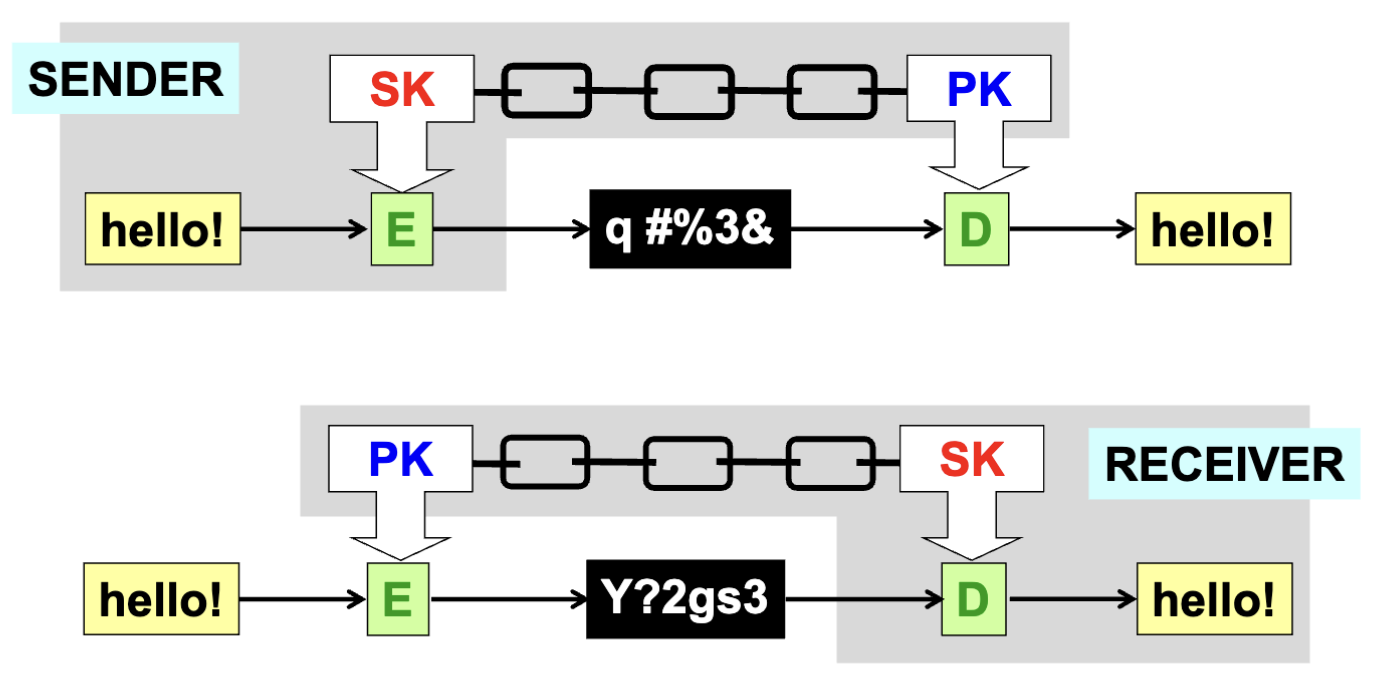
\includegraphics[width=0.5\linewidth]{Images/Cryptography/asymmCrypto.png}
    \caption{Example of asymmetric encryption}
\end{figure}


\subsection{Digital Signature - The Idea}
\begin{center}
    Authentication (but still no integrity and no repudiation).
\end{center}
\begin{tcolorbox}[colback=red!10!white, colframe=red!70!black, coltitle=white, title=Beware]
The idea has no concreteness (and actual dsig is more complex), at the exam you will explain the REAL implementation.
\end{tcolorbox}
\begin{center}
Asymmetric encryption of data made with the private key of the sender. \\ 
Look at the "Authentication by Digest and Asymmetric Encryption" section for further explanation.
\end{center}

Key features:
\begin{itemize}
    \item The idea provides data authentication.
    \item The actual digital signature offers also integrity and non-repudiation.
\end{itemize}


\begin{figure}[H]
    \centering
    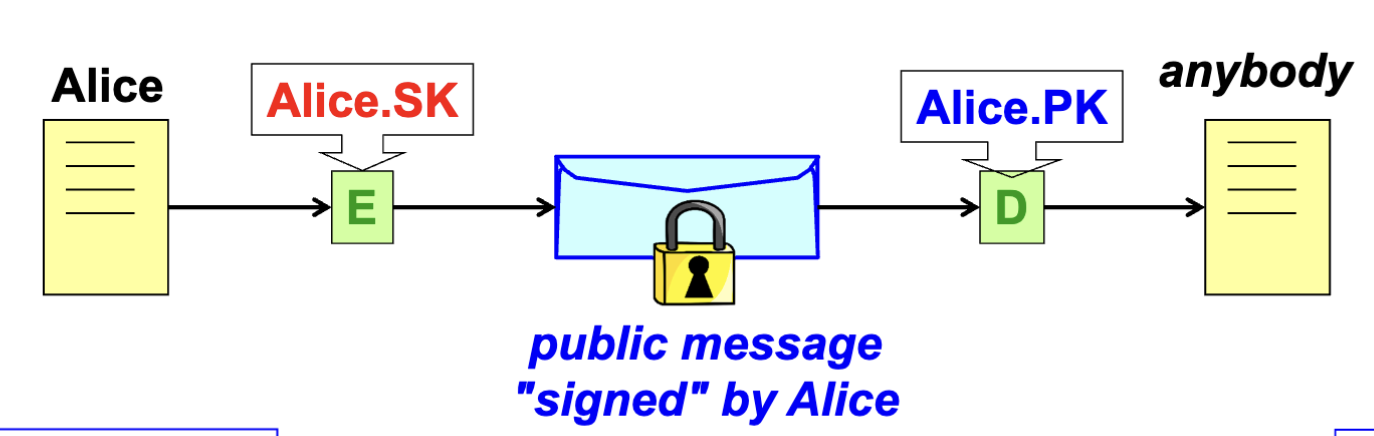
\includegraphics[width=0.5\linewidth]{Images/Cryptography/basic_digital_signature.png}
    \caption{Basic idea of digital Signature}
\end{figure}


\subsection{Asymmetric Cryptography Algorithms}
Minimum acceptable key length: 2048 bits.

\subsubsection{Rivest-Shamir-Adleman}
\begin{center}
    (RSA)
\end{center}

Its security relies on the difficulty of factoring large composite numbers.\footnote{Reference appendix A, Factorization Attack.}

\begin{center}
    \textbf{The Algorithm}
\end{center}

Main features:
\begin{itemize}
    \item Public module $N = P \cdot Q$, known to anybody.
    \begin{itemize}
        \item $P, Q$ are prime numbers, large and secret (deleted/discarded after their usage, dangerous if someone can find them!).
    \end{itemize} 
    \item Exponents:
    \begin{itemize}
        \item Public exponent: $E$. Arbitrarily chosen, $1 < E < \phi(N)$ (Euler's totient function).
        \[
            \phi(N) = (P-1) \cdot (Q-1)
        \]
        \item Private exponent: $D$. Calculated as $D = E^{-1}\cdot \mod \phi(N)$\footnote{Modulus as the remainder of the integer division.}.
    \end{itemize}
    \item Keys:
    \begin{itemize}
        \item Public key: $(N, E)$.
        \item Private key: $(N, D)$.
        \item Key length: size of the public module.
    \end{itemize}
\end{itemize}

\noindent\textcolor{Red}{Be aware:} RSA may cipher/decipher only data whose value is less than the value of the module N (it's a sort of block algorithm, with block size equal to the key size).

\noindent Main aspects:
\begin{itemize}
    \item Plaintext\_size: P < N.
    \item Encryption: $C = P^E \mod N$.
    \item Decryption: $P = C^D \mod N$.
    \item The roles of $E$ and $D$ are interchangeable.
    \[
        (C)^D \mod N = (P^D)^E \mod N = P
    \]
\end{itemize}

\begin{center}
    \textbf{Computational Optimization}
\end{center}

Usually, all public keys have E=3, 17 or 65537. Because the power operation is very easy on numbers with two bits set to one.
\begin{itemize}
    \item High speed of the encryption operation and in signature verification.
\end{itemize}
Operations involving the private key (signing and decrypting) are slow. So, the CRT (\textbf{Chinese Remainder Theorem}) is used to speed up 4x the decryption operation.
Thanks to the equivalence: 
\[
    f(x) \mod N = (f(x) \mod P)\ \&\ (f(x) \mod Q)
\]


\subsubsection{Digital Signature Algorithm}
\begin{center}
    (DSA)
\end{center}
Used for digital signature (Authentication) only: Because it uses a one-way lossy compression function, so original plaintext cannot be recovered.

Main features:
\begin{itemize}
    \item Modular exponentiation.
    \item For encryption, use the El-Gamal algorithm.
\end{itemize}

\begin{tcolorbox}[colback=red!10!white, colframe=red!70!black, coltitle=white, title=Beware]
    Algorithm based on discrete logarithms. It is mainly vulnerable due to mathematical weaknesses or implementation flaws.\footnote{Reference appendix A, Logarithmic Attacks.}
\end{tcolorbox}

\clearpage

\section{Keys Distribution}

\noindent How to share the public key:
\begin{enumerate}
    \item Exchange OOB (Out-of-bound, e.g. manually).
    \item Public-key certificate (aka digital certificate).
\end{enumerate}

In order to exchange a shared secret (symmetric key) we can use:
\begin{enumerate}
    \item Exchange OOB.
    \item Asymmetric cryptography.
    \item Diffie-Hellman (DH) key exchange.
    \item Elliptic Curve Cryptography (ECC).
\end{enumerate}

\subsection{Shared Secret Key Exchange by Asymmetric Algorithms}
Confidentiality without shared secrets is often used to send the secret key for symmetric encryption. In the top branch of the figure, X sends the encrypted message to Y using the shared key (symmetric encryption). In the bottom branch, X sends the secret key to Y using Y's public key (asymmetric encryption).

\begin{figure}[H]
    \centering
    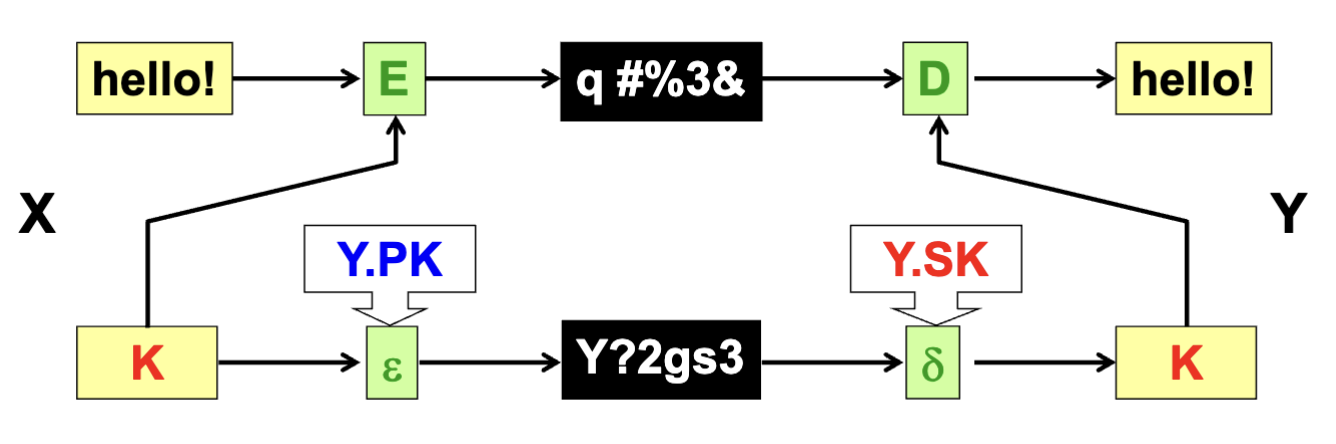
\includegraphics[width=0.7\linewidth]{Images/Cryptography/pk_exchange.png}
    \caption{Secret key exchange by asymmetric algorithms}
\end{figure}

\clearpage

\subsection{Diffie-Hellman Key Exchange}
\begin{center}
    (DH) - Modular Arithmetic.
\end{center}
Main features:
\begin{itemize}
    \item Frequently used to agree on a secret key (key agreement protocol).
    \item Resistant to sniffing attacks.
    \item If the attacker can manipulate the data then it is possible to make a man-in-the-middle attack.\footnote{Reference appendix A}
    \begin{itemize}
        \item To avoid this, the Diffie-Hellman key exchange is often combined with a digital signature algorithm (authentication).
        \item We need certificates for DH keys.
        \item Authenticated DH is MQV (Menezes-Qu-Vanstone).
    \end{itemize}
\end{itemize}

\begin{center}
    \textbf{The Algorithm}
\end{center}
\begin{multicols}{2}
    \begin{center}
        \boxed{\textbf{A}}
        \vspace{0.2cm}
        \hrule
    \end{center}

\columnbreak
\columnseprule=1pt

    \begin{center}
        \boxed{\textbf{B}}
        \vspace{0.2cm}
        \hrule
    \end{center}
    
\end{multicols}

\begin{center}
    A and B agree on two numbers: a large prime number P and a base G (typically 2,3 or 5). Such that:
    \[
        1 < G < P
    \]
    \textcolor{Blue}{(The number of bits of P is the key length)}
\end{center}

\begin{multicols}{2}
    \centering
    Arbitrarily chooses a secret number (integer) x > 0.
    \[
        X= G^x \mod P
    \]
    \columnseprule=1pt
    \columnbreak
    
    Arbitrarily chooses a secret number (integer) y > 0.
    \[
        Y= G^y \mod P
    \]
\end{multicols}

\begin{center}
    A and B exchange (publish) X and Y.
\end{center}

\begin{multicols}{2}
    \centering
    Calculates the shared secret key: \\ $K_A = Y^x \mod P$.
    
    \columnseprule=1pt
    \columnbreak

    Calculates the shared secret key: \\ $K_B = X^y \mod P$.
\end{multicols}

\vspace{1 cm}

So the shared key derived by two parties is: $K_A = K_B=G^{x\cdot y}\mod P$.

\subsection{Elliptic Curve Cryptography}
\begin{center}
    (ECC)
\end{center}
Main features:
\begin{itemize}
    \item Instead of using modular arithmetic, the operations are executed on the surface of a 2D (elliptic) curve. So, the pair of numbers is generated by the curve's equation. 
    \item Only the curve's equation is public.
    \item Digital signature: ECDSA.
    \item Key exchange: ECDH.
    \item Authenticated key agreement: ECMQV (currently patented).
    \item Key distribution: EC Integrated Encryption Scheme (ECIES).
\end{itemize}

\begin{center}
    \textbf{Arithmetics on Elliptic Curves}
\end{center}

Considering a curve: $y^2 = x^3 + ax + b \pmod{p}$ over a finite field\footnote{The arithmetic is performed over a finite field modulo a prime number  p .} $\mathbb{F}_p$.\\
With the condition\footnote{The condition ensures the curve is non-singular, meaning it does not have any cusps or self-intersections.}: $4a^3 + 27b^2 \neq 0$.\\
Compute $R=(x,y)=P+Q$ given:
\begin{itemize}
    \item $P=(x_P,y_P)$.
    \item $Q=(x_Q,y_Q)$.
\end{itemize}
$x= \lambda^2 - x_P - x_Q$ and $y= \lambda(x_P - x) - y_P$ such that the slope $\lambda$ is:
\begin{itemize}
    \item $\lambda = \frac{y_P - y_Q}{x_P - x_Q}$ if $P \neq Q$.
    \item $\lambda = \frac{3x_P + a}{2y_P}$ if $P = Q$.
\end{itemize}

\vspace{1cm}

So we can compute: Addition of two points and Multiplication of a point by a scalar.
\begin{figure}[H]
    \centering
    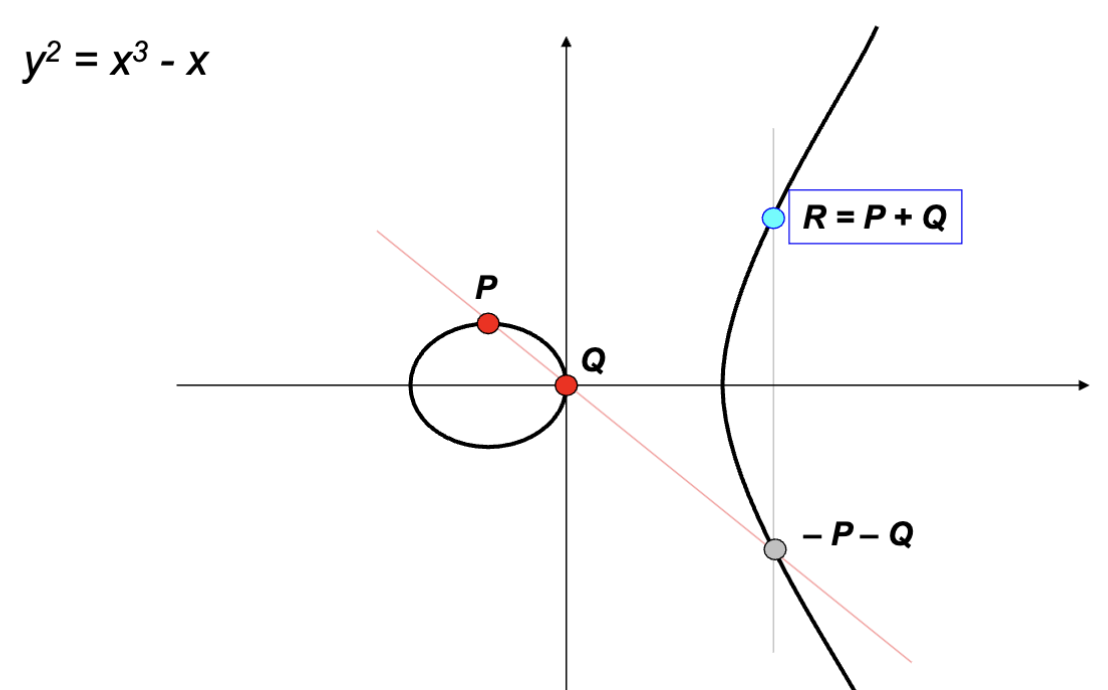
\includegraphics[width=0.5\linewidth]{Images/Cryptography/ec_arith.png}
    \caption{Elliptic Curve arithmetics}
\end{figure}

\begin{tcolorbox}[colback=blue!10!white, colframe=blue!50!white]
    Increased computational complexity can allow for shorter key lengths while maintaining the same level of security.
\end{tcolorbox}

\subsubsection{Elliptic Curve Diffie-Hellman}
\begin{center}
    (ECDH)
\end{center}

\begin{multicols}{2}
    \begin{center}
        \boxed{\textbf{A}}
        \vspace{0.2cm}
        \hrule
    \end{center}

\columnbreak
\columnseprule=1pt

    \begin{center}
        \boxed{\textbf{B}}
        \vspace{0.2cm}
        \hrule
    \end{center}
    
\end{multicols}

\begin{center}
    A and B select the same elliptic curve and a point G of its. Such that:
    \[
         G \in curve
    \]
\end{center}

\begin{multicols}{2}
    \centering
    Arbitrarily chooses a secret number x.
    \[
        X= G \cdot x
    \]
    \columnseprule=1pt
    \columnbreak
    
    Arbitrarily chooses a secret number y.
    \[
        Y= G \cdot y
    \]
\end{multicols}

\begin{center}
    A and B exchange (publish) X and Y.
\end{center}

\begin{multicols}{2}
    \centering
    Calculates the shared secret key: \\ $K_A = Y \cdot x$.
    
    \columnseprule=1pt
    \columnbreak

    Calculates the shared secret key: \\ $K_B = X\cdot y$.
\end{multicols}

\begin{tcolorbox}[colback=blue!10!white, colframe=blue!50!white]
    Computing a power would add much more complexity to the algorithm. So the shared key is computed by multiplying a point by a scalar.
\end{tcolorbox}

\section{Message Integrity}
A person that intercepts an encrypted communication cannot read it, but can modify it. So, we need to ensure the \underline{integrity} of the message.

\subsection{Cryptographic Hash Functions}

In order to ensure the integrity of a message, sender and receiver can check if the message digest is the same. The message digest is a fixed-size string mainly generated by a hash function from the message.

\vspace{0.1cm}

\noindent The digest (output of the hash function) must be:
\begin{itemize}
    \item Fast to compute.
    \item Have pre-image resistance: It is computationally infeasible to find the original message, starting from the hash (one-way function).
    \item Have collision resistance: It is computationally infeasible to find two different messages that produce the same hash.
\end{itemize}

Minimum acceptable digest length: 256 bits (balanced with a symmetric key of 128 bits).

\begin{figure}[H]
    \centering
    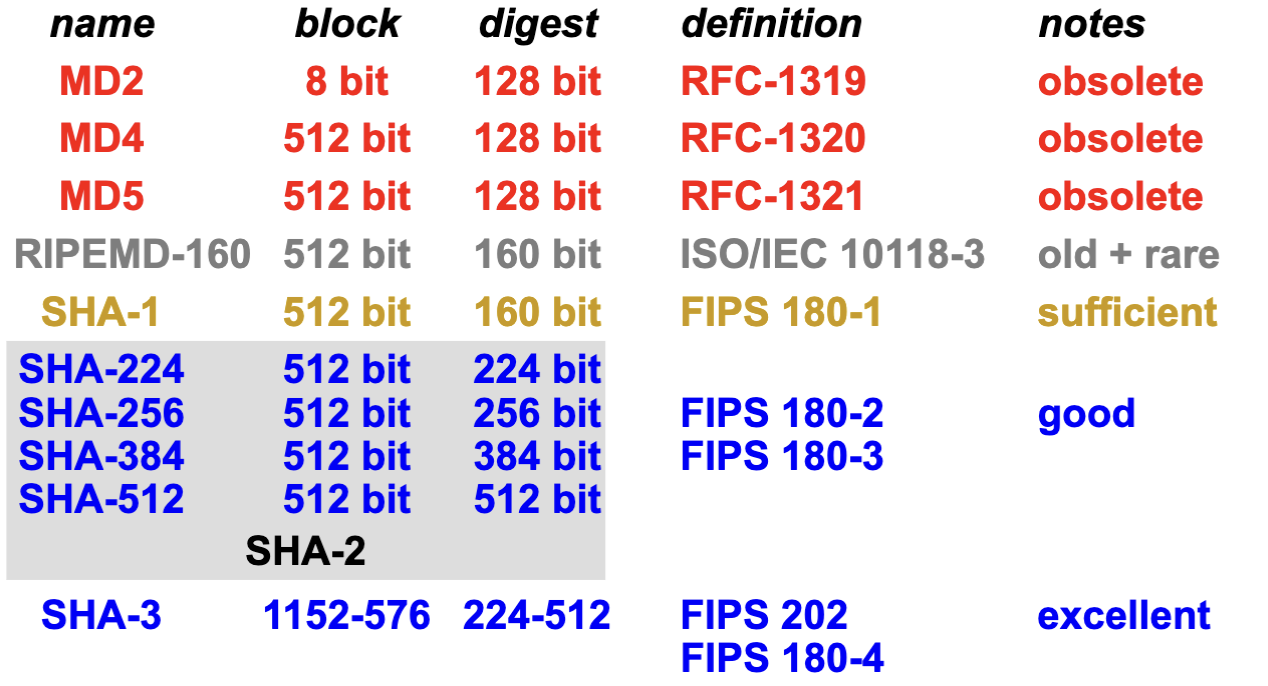
\includegraphics[width=0.5\linewidth]{Images/Cryptography/crypto_hash_functions.png}
    \caption{Cryptographic hash functions}
\end{figure}

\begin{center}
    \subsubsection*{The Algorithm}
\end{center}
Usually hash functions calculate digests through a chained process:
\begin{itemize}
    \item Split the message $M$ into $N$ blocks.
    \[
        M = M_1 || M_2 || \dots || M_N
    \]
    \item Iteratively apply a base function $f$ to each block.
    \[
        V_k = f(V_{k-1}, M_k) \quad \text{for} \quad k=1,2,\dots,N
    \]
    \[  
        \text{where} \quad V_0 = IV
    \]
    \item The final digest is the last value of the iteration $V_N$.
\end{itemize}

\begin{figure}[H]
    \centering
    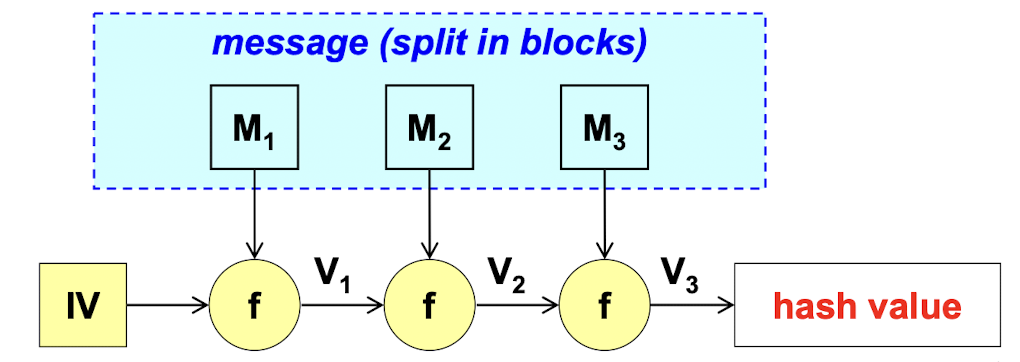
\includegraphics[width=0.5\linewidth]{Images/Cryptography/hash_f.png}
    \caption{Hash function process}
\end{figure}

\subsubsection*{Padding in Cryptographic Hash Functions}
Each function defines its own padding method.

For example, the \textbf{SHA-1} function has 512-bit blocks and uses the following padding:
\begin{itemize}
    \item Block size $B = 512$ bits and fragment (if the message length is not a multiple of 512 bits) size $L (< B)$ bits.
    \item Append a bit with value 1, followed by $K$ bits with value 0, where $K = B - L - 64$.
    \item The last 64 bits are the length of the original message.
\end{itemize}


\begin{tcolorbox}[colback=red!10!white, colframe=red!70!black, coltitle=white, title=Beware]
SHA-2 and SHA-3 are families of cryptographic hash functions. You must always specify the exact algorithm (SHA-256, SHA-512, etc.).
\end{tcolorbox}

\subsubsection*{SHA-2 Family}
\begin{center}
    (Secure Hash Algorithm 2)
\end{center}
SHA-2 is a family of cryptographic hash functions that includes SHA-224, SHA-256, SHA-384, SHA-512. The SHA-256 and SHA-512 algorithms are the most commonly used. As a quick fix after the SHA-1 attack, the SHA-2 family was developed by making the digest size larger.

SHA-224/-384 are the truncation of SHA-256/-512. 

\subsection{Digest Length}
The length of the digest is important because it determines the probability of a collision \newline (= \textcolor{Blue}{Aliasing}). 

If the algorithm is well-designed, and generates a digest of $N$ bits, \\ the probability of aliasing is:
\[
    P_A \propto \frac{1}{2^{N}}
\]
\dots thus, digests with many bits are required to avoid aliasing.

\subsection{The Birthday Paradox}
\begin{center}
    (Collision Probability, basic problem of hashing)
\end{center}

\begin{multicols}{2}
    The birthday paradox is a probability problem that asks how many people need to be in a room for the probability of two people sharing the same birthday to be greater than 50\%. The same concept applies to hash functions: the probability of two different messages having the same hash is higher than expected.

    \vspace{0.5cm}

    \begin{center}
        Reference Appendix A for the Birthday Attack.
    \end{center}

\columnbreak

    \begin{figure}[H]
        \centering
        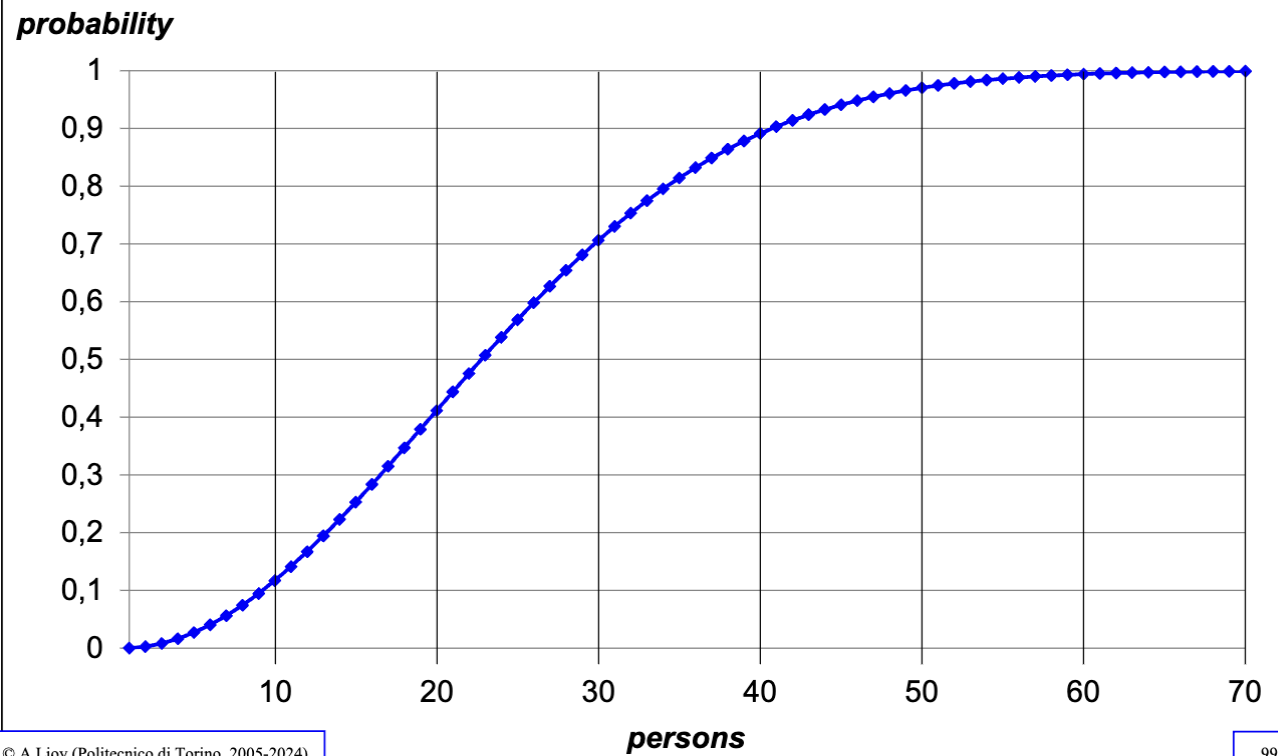
\includegraphics[width=\linewidth]{Images/Cryptography/bd_paradox.png}
        \caption{Birthday Paradox}
    \end{figure}
\end{multicols}



    \textbf{An $N$-bit hash function is considered insecure when more than $2^{N/2}$ digests are generated, because the probability to have two messages with the same digests is greater than 50\%. }

\textcolor{red}{Be aware:} A cryptosystem is balanced when the encryption and digest algorithms have the same resistance to attacks. SHA-256 and SHA-512 have been designed for use respectively with AES-128 and AES-256.

\begin{tcolorbox}[colback=red!10!white, colframe=red!70!black, coltitle=white, title=Beware]
    A system is only as secure as its weakest link.
\end{tcolorbox}

\subsubsection*{SHA-3 Family}
\begin{center}
    (Secure Hash Algorithm 3, named Keccak (pronounce: \textit{catch-ack}))
\end{center}
The SHA-3 family was developed as a backup to SHA-2 in case of a successful attack. The design of SHA-3 is completely different from that of SHA-2 and SHA-1.

\vspace{0.5cm}

\noindent Key features:
\begin{itemize}
    \item Elegant design.
    \item Run well on many computing devices.
    \item Higher performance in hardware implementations than SHA-2.
\end{itemize}

\begin{figure}[H]
    \centering
    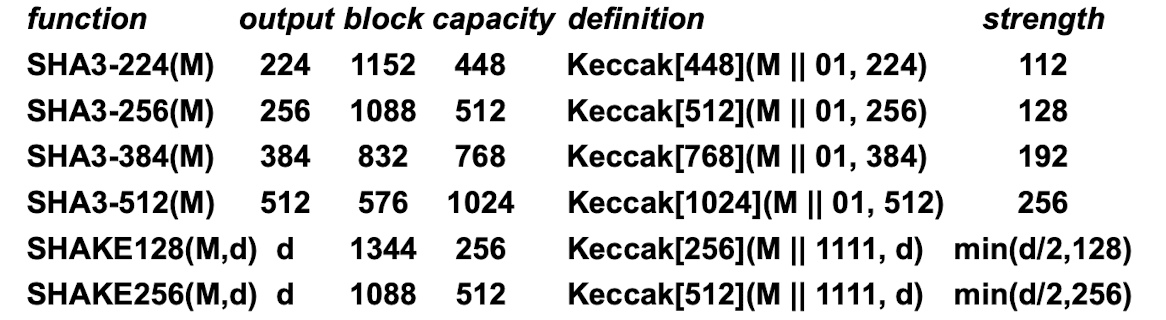
\includegraphics[width=0.5\linewidth]{Images/Cryptography/sha_3.png}
    \caption{SHA-3 family}
\end{figure}

\vspace{0.5cm}

And more (NIST SP: 800-185) SHA-3 family includes:
\begin{itemize}
    \item cSHAKE128, cSHAKE256: Customizable domain parameters.
    \item KMAC128, KMAC256: Keyed digest functions.
    \item TupleHash: Hash of a tuple, where sequence matters.
    \item ParallelHash: Fast hashing for multicore processors.
\end{itemize}

\section{Key Derivation Functions}
\begin{center}
    (KDF)
\end{center}
A cryptographic key must be random (each bit has a 50\% probability of being 0 or 1), but users typically choose passwords (or better, \textbf{passphrases}) guessable and not random. So the KDF is used to derive a key from a passphrase.

Main elements of a Key Derivation Function:
\[
    \text{KDF (P, S, I)} = \text{DerivedKey}
\]

\begin{itemize}
    \item P: Passphrase (e.g. password).
    \item S: Salt, to make K difficult to guess given P.
    \item I: how many times (Iterations) the function is applied (to slow down the computation and make life complex for attackers).
\end{itemize}

\vspace{0.2cm}

Some KDF based upon cryptographic hash functions:
\begin{itemize}
    \item PBKDF2 (Password-Based Key Derivation Function 2, RFC-2898).
    \begin{itemize}
        \item Uses SHA-1, $|S| \ge 64$, $|I| \ge 1000$.
    \end{itemize}
    \item HKDF (HMAC-based Extract-and-Expand Key Derivation Function, RFC-5869).
\end{itemize}

\subsection{Password-Based Key Derivation Function 2}
\begin{center}
    (PBKDF2, RFC-8018)
\end{center}

Main features:
\begin{itemize}
    \item Replaces PBKDF1, due to key length limitations ($\le 160$ bits).
\end{itemize}
Main elements to compute the derived key (DK):
\[
    \text{DK} = \text{PBKDF2 (PRF, PWD, Salt, C, dkLen)}
\]
\begin{itemize}
    \item PRF: Pseudo-Random Function with output length hLen(e.g. a keyed HMAC = HMAC-SHA-1).
    \item PWD: Password.
    \item Salt: Random value.
    \item C: Number of iterations desired.
    \item dkLen: Desired length of the derived key.
\end{itemize}

The Derived Key (DK) is constructed by concatenating components $T_1, T_2, \dots, T_{\lceil dkLen/hLen \rceil}$\footnote{$\lceil dkLen / hLen \rceil$  determines the number of components needed to reach or exceed the target key length.}, where each $|T_i| = hLen$.

\subsubsection*{PBKDF2 Parameters and Applications}
In WPA2 (Wi-Fi Protected Access 2), PBKDF2 is a core part of the 4-Way Handshake process. It is used to derive cryptographic keys securely from the Wi-Fi password to ensure encryption and integrity.
\[
    \text{(WPA2) DK = PBKDF2 (HMAC-SHA1, PSK, SSID, 4096, 256)}
\]

\clearpage
\section{Integrity, Authentication and Reliability Messages}
The following codes are sent with the message to ensure its integrity, authentication, and reliability, respectively:
\begin{itemize}
    \item MIC (Message Integrity Code): Computed using some data and a MIC function (can be a cryptographic hash function) to provide integrity (simil checksum). \textcolor{Blue}{Integrity}
    \item MAC (Message Authentication Code): Computed using a shared key, some data, and a MAC function (can be a cryptographic hash function, would be a keyed-digest). \textcolor{Blue}{Integrity and Authentication}
    \item MID (Message IDentification): A unique identifier to ensure the message is not duplicated (partially\footnote{Attackers can still forge messages based on the weaknesses of an identifier (management and synchronization.)} avoid replay attacks). \textcolor{Blue}{Reliability}
\end{itemize}

\begin{tcolorbox}[colback=red!10!white, colframe=red!70!black, coltitle=white, title=Beware]
    The added message should be encrypted; otherwise, a man-in-the-middle (MITM) attacker could modify both the hash and the message on-the-fly, bypassing integrity checks.
\end{tcolorbox}

\section{Keyed-Digest}
\begin{center}
    Possible implementation of a MAC.

    Authentication + Integrity.
\end{center}
\textcolor{Red}{No confidentiality!! The key has not this purpose in this mechanism.}

\hfill

A keyed-digest is obtained by applying a hash function to the message concatenated with a shared secret key. 
\begin{itemize}
    \item The sender sends the message and the keyed-digest to the receiver. 
    \item The receiver computes a keyed-digest of the same data (using the same shared key). 
    \item \textcolor{Blue}{Conclusion to say: }If the two digests match, the message is considered authentic (because used the same shared key) and integral (data not altered).

\end{itemize}
\begin{tcolorbox}[colback=red!10!white, colframe=red!70!black, coltitle=white, title=Beware]
If the check fails, we don't know if the message was altered or if the key was wrong. So the message and the keyed-digest must be discarded.
\end{tcolorbox}

\begin{multicols}{2}
    \raggedcolumns
    Advantages:
    \begin{itemize}
        \item Only one operation (hash).
        \item Few additional data (little overhead).
        \item Authentication + Integrity.
    \end{itemize}
\columnbreak

\begin{figure}[H]
    \centering
    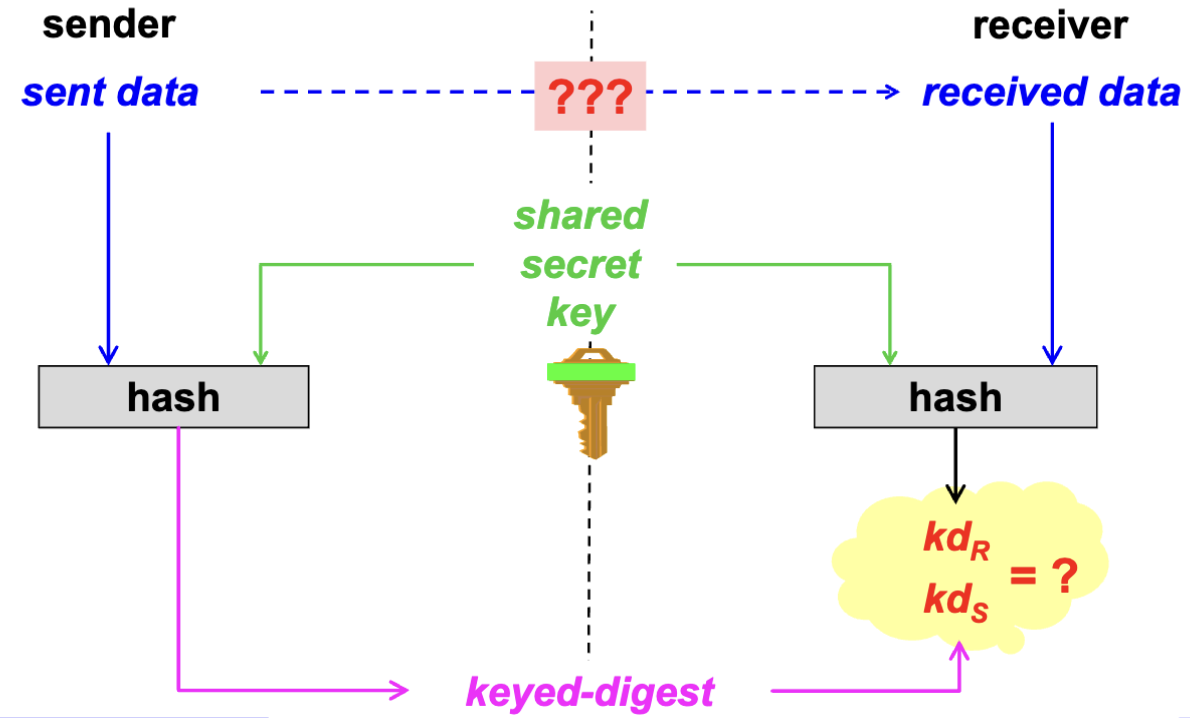
\includegraphics[width=\linewidth]{Images/Cryptography/keyed_digest.png}
    \caption{Keyed-Digest process}
\end{figure}
\end{multicols}

\subsection{Hash-based Message Authentication Code}
\begin{center}
    (HMAC) - RFC-2104 (also FIPS-198) - The only secure standard available.
    \\ Key-based method used to verify both the integrity and authenticity of a message  M .
\end{center}

\[
\text{HMAC-H} = \text{H}\big((K' \oplus \text{opad}) \, \| \, \text{H}((K' \oplus \text{ipad}) \, \| \, M)\big)
\]

\begin{itemize}
    \item H: Hash function (e.g. SHA-256).
    \item M: Message.
    \item K: The original secret key shared between two parties.
    \begin{itemize}
        \item $K' = H(K)$\quad if $|K| > B$.
        \item $K' = K$\quad\ \ \quad if $|K| \le B$.
    \end{itemize}
    \item K': The block-sized key derived from  K.
    \begin{itemize}
        \item 0-padded up to $B$ bytes\quad if $|K'| < B$.
    \end{itemize}
    \item ipad: Inner padding (0x36 repeated B times).
    \item opad: Outer padding (0x5C repeated B times).
\end{itemize}


\subsection{CBC-MAC}
\begin{center}
    (Cipher Block Chaining Message Authentication Code)
\end{center}
\textcolor{Red}{No for confidentiality!! No encryption of data.}

Main features:
\begin{itemize}
    \item Exploits a block-oriented symmetric encryption algorithm.
    \item CBC mod with null IV.
    \item Takes as MAC the last encrypted block.
\end{itemize}

\begin{center}
    \textbf{The Algorithm}
\end{center}
The message $M$ is divided into $N$ blocks $M_1, M_2, \dots, M_N$.
\begin{itemize}
    \item $V_0 = IV = 0$.
    \item $V_i = enc(V_{i-1} \oplus M_i, K)$ \quad \quad for ($i=1,2,\dots,N$).
    \item The MAC (aka CBC-MAC) is the last block $V_N$.
\end{itemize}

\subsubsection*{CBC-MAC Insecurity}
Reasons:
\begin{itemize}
    \item Secure only for fixed length messages (for other cases use CMAC or OMAC).
\end{itemize}
Possible attack against variable-length messages:
    \begin{itemize}
        \item If you have a CBC-MAC tag $t$ for a message $M$ and a tag $t'$ for another message $M'$, an attacker can construct a new message $M''$ such that the tag for $M''$ is valid without knowing the key $K$ (forgery attack).
        
\end{itemize}
\begin{center}
    Operational proof
\end{center}
    \begin{itemize}
        \item If I create a new message $M''$ as follows:
        \[
            M'' = M \, || \, (M'_1 \oplus t) \, || \, M'_2 \, || \, \dots \, || \, M'_N
        \]
        \begin{itemize}
            \item $M'_1 \oplus t$ modifies the first block of M' using the previous tag t to “cancel out” contributions.
        \end{itemize} 
        \[
            t'' = \text{CBC-MAC}(M'', K) = t'
        \]
        \item The resulting CBC-MAC tag for $M''$ ends up being $t'$, the tag of $M'$, effectively forging the message without knowing the key.
    \end{itemize}

\section*{Performances of Cryptographic Algorithms}
On large data, the computational effort of the cryptographic algorithms is:
\begin{figure}[H]
    \centering
    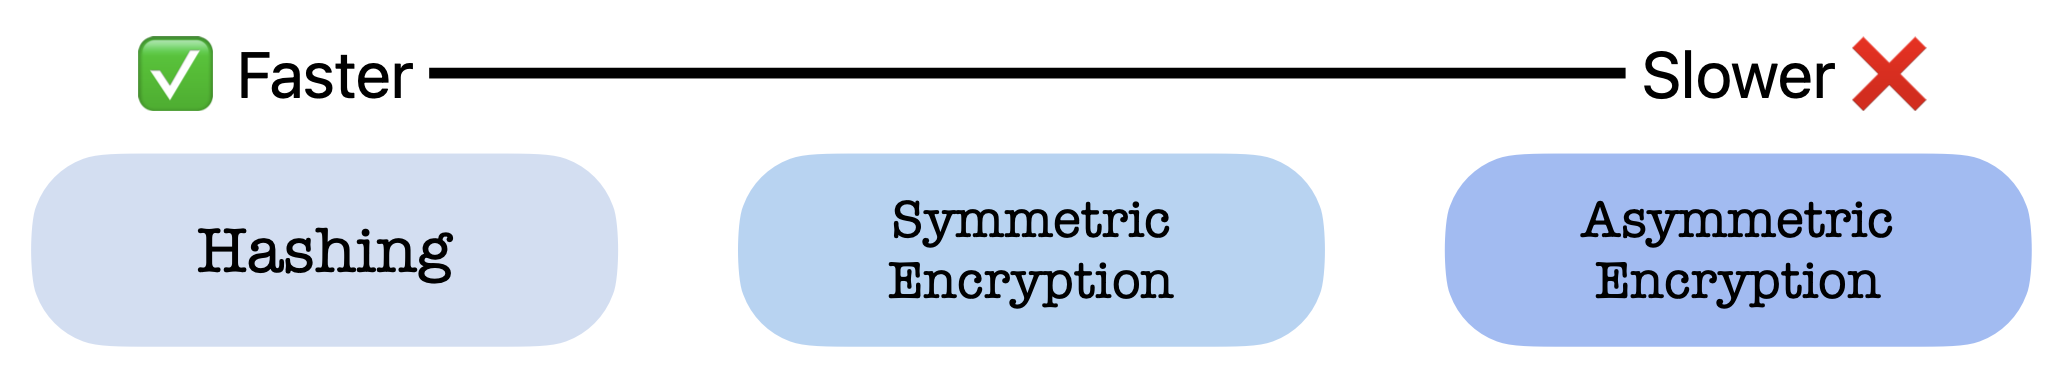
\includegraphics[width=0.7\linewidth]{Images/Cryptography/velocity.png}
    \caption{Hashing, Symmetric and Asymmetric Cryptography - Computational Effort}
\end{figure}

\clearpage 
\section{Integrity and Secrecy of Data}
\begin{center}
    (Confidentiality, Integrity and Authenticity)
\end{center}
We obtain:
\begin{itemize}
    \item Secrecy (confidentiality) from encryption with a key $K_1$.
    \item Authenticity, and integrity, from a MAC with a key $K_2$.
\end{itemize}

\hfill 

\begin{center}
    \textbf{Modalities}
\end{center}

    \begin{multicols}{2}

        \subsection*{Authenticate and Encrypt}
    \begin{center}
        A\&E
    \end{center}
    \[
        enc(K_1, M) \, || \, \text{MAC}(K_2, M)
    \]
    Key points:
    \begin{itemize}
        \item May leak info about the plaintext.
        \item Used by SSH.
        \item You will know if the message is corrupted at the end of the decryption.
        \item Insecure unless performed in a single step.
    \end{itemize}
\columnbreak

    \subsection*{Authenticate then Encrypt}
    \begin{center}
        AtE
    \end{center}
    \[
        enc(K_1, M \, || \, \text{MAC}(K_2, M))
    \]
    Key points:
    \begin{itemize}
        \item No info leakage.
        \item Used by SSL/TLS.
        \item Secure only with CBC or stream encryption.
    \end{itemize}
\end{multicols}

\begin{center}
    \subsection*{Encrypt then Authenticate}
    \begin{center}
        EtA \\ Best solution.
    \end{center}
    \[
        enc(K_1, M) \, || \, \text{MAC}(K_2, enc(K_1, M))
    \]
\end{center}

Key points:
\begin{itemize}
    \item Can avoid decryption if MAC is wrong
    \item Used by IPsec.
    \item The most secure mode, but beware of implementation errors (e.g., always include the  IV  and algorithms in the MAC).
\end{itemize}

\begin{tcolorbox}[colback=red!10!white, colframe=red!70!black, coltitle=white, title=Beware]
    Improper combination of secure algorithms may lead to an insecure result !
\end{tcolorbox}
A modern solution to that is Authenticated Encryption (AE) that combines encryption and authentication in a single operation.

\subsection{Authenticated Encryption}
\begin{center}
    (AE)
\end{center}
A single operation for privacy and authentication/integrity.

Key features:
\begin{itemize}
    \item Just one key and one algorithm.
    \item Better speed.
    \item Less error likelihood in combining the two functions.
\end{itemize}

\subsubsection{Infinite Garble Extension}
\begin{center}
    (IGE - for Authenticated Encryption)
\end{center}
A mode of operation for block ciphers that provides both confidentiality and authenticity.

\[
    C_i = P_{i-1} \oplus enc(K_, C_{i-1} \oplus P_i) \quad \text{for} \quad i=1,2,\dots,N \text{ blocks}
\]
\[
    C_1 = IV \oplus enc(K_, P_1 \oplus enc (K', IV))
\]

\begin{figure}[H]
    \centering
    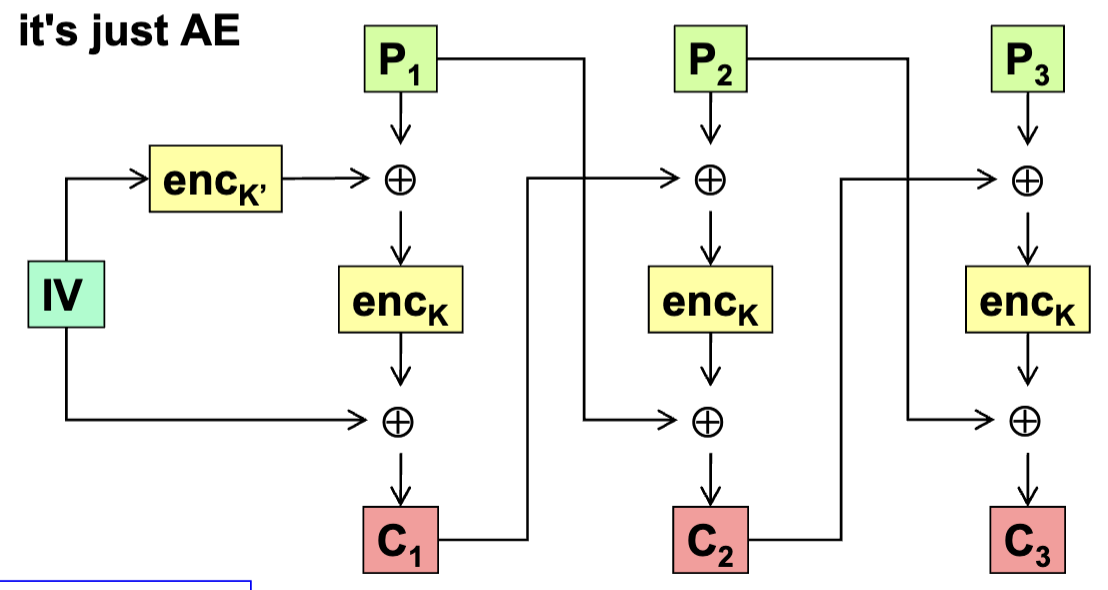
\includegraphics[width=0.5\linewidth]{Images/Cryptography/AE.png}
    \caption{Infinite Garble Extension process}
\end{figure}

\clearpage
\subsection{Authenticated Encryption with Associated Data Schema}
\begin{center}
    (AEAD - Authenticated Encryption with Associated Data)
\end{center}
\begin{tcolorbox}[colback=red!10!white, colframe=red!70!black, coltitle=white, title=Beware]
    AEAD is not a single algorithm but a cryptographic scheme that combines encryption and authentication. 
\end{tcolorbox}
Due to its Authenticated Encryption (AE) nature, it performs both encryption (confidentiality) and authentication (integrity and authenticity) in a single operation. AEAD ensures that any modification to the ciphertext or associated data is detectable.

\begin{figure}[H]
    \centering
    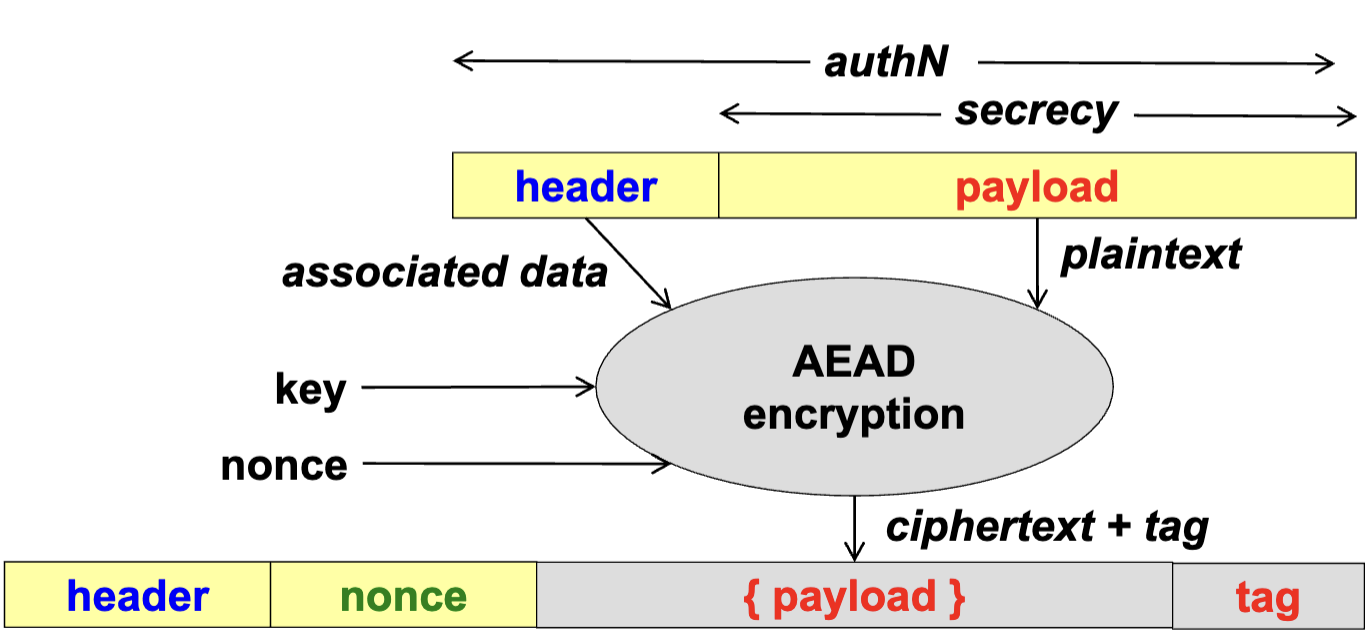
\includegraphics[width=0.6\linewidth]{Images/Cryptography/aead.png}
    \caption{AEAD scheme}
\end{figure}

\subsection{AE Standards}
Many are issued by NIST and IETF:
\begin{itemize}
    \item GCM (Galois/Counter Mode).
    \item CCM (CTR mode with CBC-MAC): off-line double-pass, the slowest one.
    \item EAX (Encrypt-then-Authenticate-then-Encrypt with X translation = CTR + OMAC): on-line double-pass AEAD. Slow but small (uses just the encryption block) so very good for constrained systems.
    \item OCB (Offset Codebook Mode): the fastest one, on-line single-pass AEAD. GPL patented so scarcely used, now free but for military uses.
    \item AESKW (AES Key Wrap).
    \item Encrypt-then-MAC (EtM).
\end{itemize}
\begin{tcolorbox}[colback=blue!10!white, colframe=blue!50!white]
Double-pass is 2x slower than single-pass (in software).
\end{tcolorbox}

\clearpage

\subsubsection{Galois/Counter Mode as AEAD}
\begin{center}
    GCM as an example of AEAD. \\ Defined for encryption algorithms with 128-bit block size.
\end{center}
Is the most popular, on-line single-pass AEAD, parallelizable.
\[
    \text{(C, T)} = \text{GCM\_enc}(K, IV, A, P)
\]
\begin{itemize}
    \item Outputs:
    \begin{itemize}
        \item $C$: Ciphertext, with same size as $P$.
        \item $T$: Authentication Tag, with size $[1, ..., 2^{128}]$ bits.
    \end{itemize}
    \item $IV$: Initialization Vector, with size $[1, ..., 2^{64}]$ bits (96 bits is common).
    \item $P$: Plaintext, with size $[1, ..., 2^{39}-256]$ bits.
    \item $A$: Associated Data, not encrypted but authenticated, with size $[1, ..., 2^{64}]$ bits.
    \item $K$: Key.
\end{itemize}

If the authentication is OK then it is possible to decrypt the message.
\[
    \text{P} = \text{GCM\_dec}(K, IV, A, C, T)
\]
\begin{tcolorbox}[colback=blue!10!white, colframe=blue!50!white, title=Output of decryption]
    If the authentication is OK then the output is the plaintext, otherwise a special value FAIL is returned.
\end{tcolorbox}
Is present in openssl:
\begin{itemize}
    \item For encryption: ciphertext+authentication-tag generation.
    \item For decryption: first computes the authentication tag and then decrypts the ciphertext if the tag is OK (matches the one in input).
    \item Fast on Intel architecture using AES-NI for encryption and PCLMULQDQ for the tag.
\end{itemize}

\subsubsection{CTR mode with CBC-MAC as AEAD}
\begin{center}
    CCM as an example of AEAD. \\ Defined for encryption algorithms with 128-bit block size.
\end{center}
First an authentication tag of the plaintext and associated data is calculated using CBC-MAC. Then the plaintext and associated data are encrypted using CTR mode. Then the plaintext and the tag are (separately) encrypted using CTR mode.

\subsubsection{AES Key Wrap}
\begin{center}
    AESKW - RFC-3394 \\ Only for keys, not data.
\end{center}
Assumptions:
\begin{itemize}
    \item The protocol encrypts/decrypts a key for storage/transmission.
    \item The key is a multiple of 64 bits.
    \item Generates also a 64-bit authentication tag.
\end{itemize}

\begin{center}
    \textbf{The Operations}
\end{center}
\begin{enumerate}
    \item KEK (Key Encryption Key) is the key used to encrypt/decrypt the key.
    \item CEK (Content Encryption Key) is the key to be encrypted/decrypted.
    \item {CEK} + tag = AESKW\_enc(KEK, CEK).
    \item CEK (or FAIL) = AESKW\_dec(KEK, {CEK} + tag).
\end{enumerate}
This protocol, unlike normal AE algorithms, is simple (e.g. no RNG as in GCM needed, or no asymmetric encryption) and supports in-place encryption/decryption.

\subsubsection{ASCON}
\begin{center}
    Used for encryption, AEAD, and hashing.
\end{center}
NOT to replace AES or SHA3, but to be used in constrained (lightweight) environments (e.g. IoT).
\begin{center}
    \textbf{For AEAD}
\end{center}

\begin{table}[H]
    \centering
    \begin{tabular}{lccccccc}
        \toprule
        \textbf{} & \textbf{key} & \textbf{nonce} & \textbf{tag} & \textbf{rate} & \textbf{capacity} & \textbf{pa} & \textbf{pb} \\
        \midrule
        ASCON-128  & 128 & 128 & 128 & 64  & 256 & 12 & 6 \\
        ASCON-128a & 128 & 128 & 128 & 128 & 192 & 12 & 8 \\
        \bottomrule
    \end{tabular}
\end{table}

\begin{center}
    \textbf{For Hashing}
\end{center}
\begin{table}[H]
    \centering
    \begin{tabular}{lcccccc}
        \toprule
        \textbf{} & \textbf{output} & \textbf{rate} & \textbf{capacity} & \textbf{pa} & \textbf{pb} \\
        \midrule
        ASCON-hash  & 256       & 64  & 256 & 12 & 12 \\
        ASCON-xof   & arbitrary & 64  & 256 & 12 & 12 \\
        ASCON-hasha & 256       & 64  & 256 & 12 & 8  \\
        ASCON-xofa  & arbitrary & 64  & 256 & 12 & 8  \\
        \bottomrule
    \end{tabular}
\end{table}
\begin{tcolorbox}[colback=blue!10!white, colframe=blue!50!white]
pa and pb are the number of rounds for the permutation and the number of rounds for the key schedule, respectively. The higher the number of rounds, the higher the security but also the computational effort.
\end{tcolorbox}

\subsection{AE Applications}
Here are listed some applications of AE:
\begin{itemize}
    \item TLS-1.3 (Transport Layer Security) uses GCM and CCM.
    \item 802.11i (wi-fi) uses CCM.
    \item ZigBee uses CCM* (a variant of CCM, = CCM + auth-only + enc-only).
\end{itemize}

\section{Authentication by Digest and Asymmetric Encryption}
\begin{center}
    (Real implementation of Digital Signatures)
\end{center}
The sender sends the message digest encrypted with the private key. The receiver decrypts the digest with the public key of the sender and compares it with the digest of the message. If they match, the message is authentic.
\begin{verbatim}
    Sender: 
        signedDigest = enc(hash(Message), S.SecretKey)

    Sender > Receiver:
        Message, signedDigest 

    Verifier:
        digest = dec(signedDigest, S.PublicKey)
        hash(Message) == digest ? OK : ALARM
\end{verbatim}

Those who know the public key can compare the transmitted digest with the digest calculated on the received data. It's the basis of digital signatures !! 


\clearpage

\subsection{Digital Signature}
\begin{center}
    The technical basis for digital signatures.

    Authentication + Integrity + Non-repudiation.
\end{center}
\begin{center}
    \textbf{The Algorithm}
\end{center}
The digital signature process involves creating a secure and verifiable way to ensure the authenticity, integrity, and non-repudiation of digital data. The process is as follows:
\begin{enumerate}
    \item The sender generates pair of cryptographic keys (PublicKey and SecretKey).
    \item A cryptographic \textbf{hashing} algorithm is applied to the data (message or file) to obtain a hash value.
    \item The private key is used to \textbf{encrypt} this hash value, producing the digital signature (signed hash).
    \item The signed data (original data + digital signature) is sent to the receiver.
    \item The receiver uses the sender's public key to decrypt the signature, in order to obtain the digest to verify.
    \item The receiver applies the same hashing algorithm to the received message/data.
    \item If the decrypted hash matches the hash computed locally, the digital signature is valid. This verifies:
    \begin{itemize}
        \item Authenticity: The message came from the expected sender.
        \item Integrity: The data has not been altered.
        \item Non-repudiation: The sender cannot deny having sent the message (due to the use of its own private key).
    \end{itemize}
\end{enumerate}
\begin{tcolorbox}[colback=red!10!white, colframe=red!70!black, coltitle=white, title=Beware]
In order to check the integrity of the message, the receiver must have the public key of the sender. The public key won't stay the same forever. It can be changed, so the verifier must have a way to know the new public key.
\end{tcolorbox}

\begin{figure}[H]
    \centering
    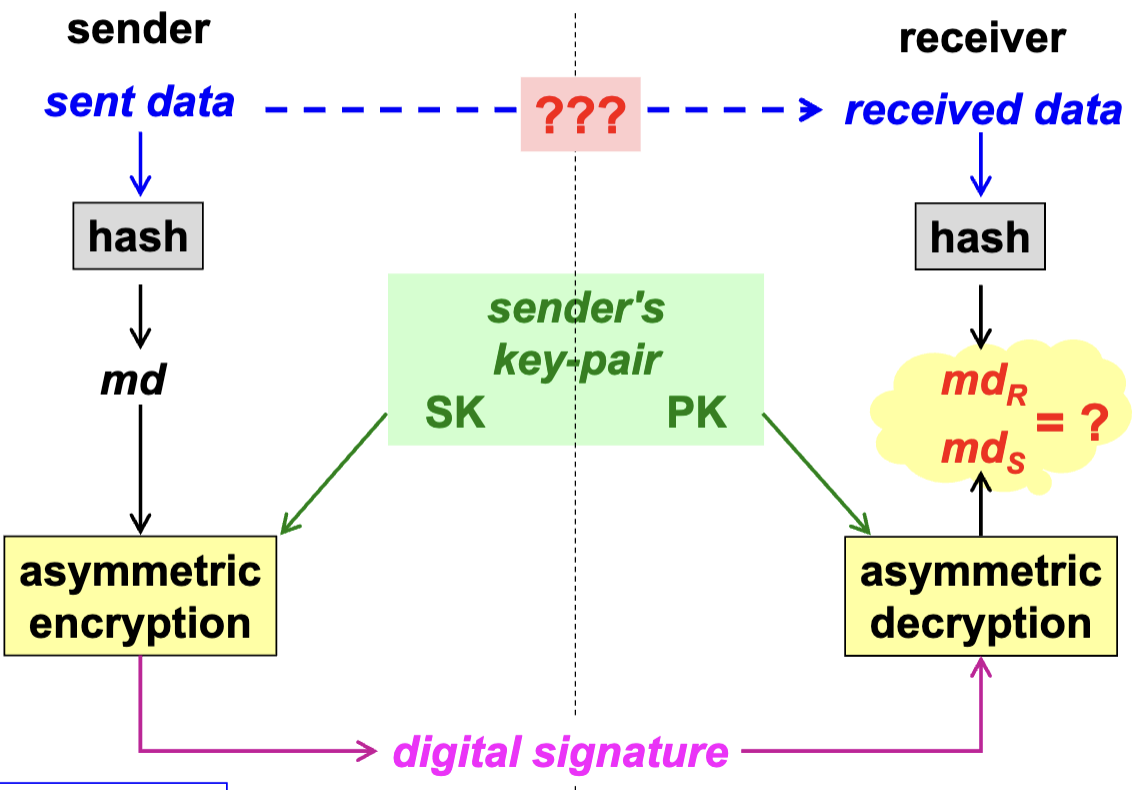
\includegraphics[width=0.4\linewidth]{Images/Cryptography/ds.png}
    \caption{Digital Signature transmission}
\end{figure}
\begin{tcolorbox}[colback=red!10!white, colframe=red!70!black, coltitle=white, title=For the Exam]
    The sender is sending the data + digital signature (encrypted hash of the message) to the receiver. 
    
    \vspace{0.2cm}
    
    Whether the manipulation happen in the data or in the digital signature, the receiver will detect it (and reject everything).
\end{tcolorbox}


\begin{center}
    \textbf{Signature Verification for Stored Data}
\end{center}

The mechanism seen above is valid also for storing data. The data is stored with the digital signature. When the data is read, the digital signature is decrypted and compared with the hash of the data. If they match, the data is authentic.
\begin{tcolorbox}[colback=blue!10!white, colframe=blue!50!white]
Once the data are signed, even if they are store in a public place, the verifier can verify the integrity of the data.
\end{tcolorbox}

\begin{figure}[H]
    \centering
    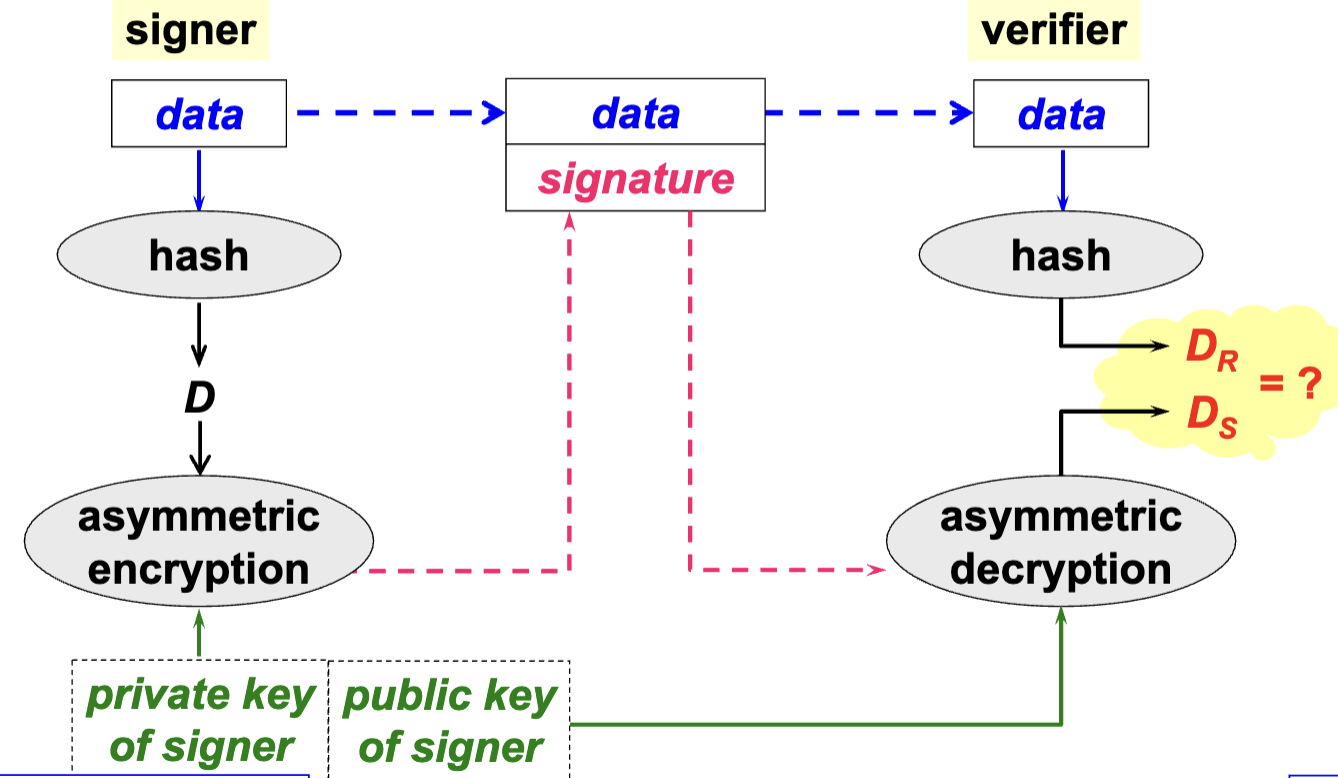
\includegraphics[width=0.6\linewidth]{Images/Cryptography/ds_storing.png}
    \caption{Digital Signature stored with the data}
\end{figure}

\subsubsection*{Digital Signature and Handwritten Signature}
\begin{multicols}{2}

    Digital signature: \\ Authentication + Integrity.
    \begin{itemize}
        \item Better because it is tightly linked to the data.
        \item Each user does not have a digital signature but a private key, which can be used to generate an infinite number of digital signatures (one for each document).
    \end{itemize}
    \columnbreak

    

    Handwritten signature: \\ Only Authentication.
    
\end{multicols}

\clearpage

\subsection{Authentication and Integrity Analysis}


\begin{multicols}{2}

    \textbf{The use of a shared secret for providing Authentication and Integrity (MAC)}:
    \begin{itemize}
        \item Useful only for the receiver.
        \item Cannot be used as a proof without disclosing the secret key.
        \item Does not provide non-repudiation.
    \end{itemize}
\columnbreak

\textbf{The use of asymmetric encryption for providing Authentication and Integrity (Digital Signature)}:
\begin{itemize}
    \item Applied only to the digest (because of the computational effort).
    \item Can be used as a formal proof-of-origin.
    \item Provides non repudiation.
\end{itemize}
\end{multicols}



\section{Public Key Infrastructure}
\begin{center}
    (PKI)
\end{center}
The PKI provides a framework for managing digital certificates and public-key encryption.

\subsection{Public Key Certificate}
\begin{center}
    Definition: \\ A data structure used to securely bind a public key to some attributes.
\end{center}

Typically, it binds a key to an identity, but other associations are possible too (e.g. IP address, domain name, etc.). The certificate is signed by a trusted third party, the Certificate Authority (CA), to ensure the authenticity of the binding. The certificate has a limited lifetime, after which it must be renewed. Can be revoked on request both by the user and the issuer.

\vspace{0.5cm}

Formats for public key certificates:
\begin{itemize}
\item X.509:
\begin{itemize}
\item v1: Initial version.
\item v2: Enhanced version introduced by ISO.
\item v3: Most commonly used version, combining ISO and IETF standards.
\end{itemize}
\item Non X.509:
\begin{itemize}
\item PGP (Pretty Good Privacy).
\item SPKI (Simple Public Key Infrastructure, IETF).
\end{itemize}
\item PKCS\#6 (Public Key Cryptography Standard \#6):
\begin{itemize}
\item RSA certificates, partially compatible with X.509.
\item Now considered obsolete.
\end{itemize}
\end{itemize}

\clearpage 
\subsubsection{X.509 Certificate}
\begin{center}
    The most common format for public key certificates.
\end{center}
\begin{center}
    \textbf{The Structure}
\end{center}

\begin{multicols}{2}

    \begin{itemize}
        \item Version: The version of the X.509 standard.
        \item Serial Number: A unique number assigned by the CA.
        \item Signature Algorithm: The algorithm used by the CA to sign the certificate.
        \item Issuer: The entity that issued the certificate.
        \item Validity: The period during which the certificate is valid.
        \item Subject: The entity to which the certificate is issued. Written with its Distinguished Name (DN).
        \item Subject Public Key Info: The public key of the subject.
        \item CA Signature: The digital signature of the CA.
    \end{itemize}

\columnbreak

    \begin{figure}[H]
        \centering
        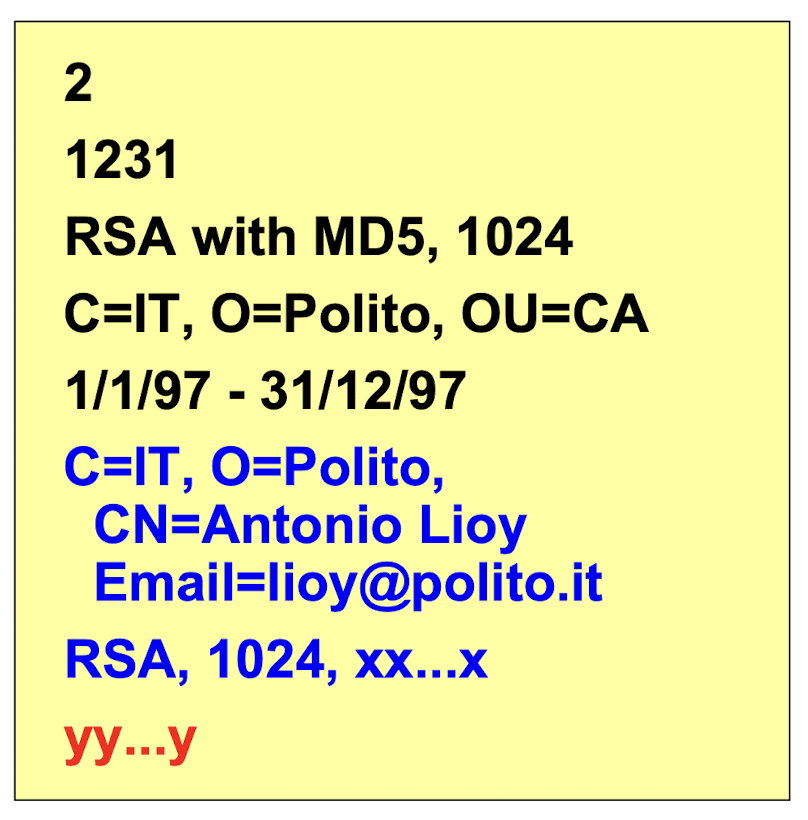
\includegraphics[width=\linewidth]{Images/Cryptography/x509.png}
        \caption{X.509 Certificate structure}
    \end{figure}
\end{multicols}

\subsection{Certificate Revocation}
Any certificate can be revoked before its expiration date:
\begin{itemize}
\item At the request of the owner (subject).
\item Unilaterally by the issuer (issuer).
\end{itemize}
When verifying a signature, the receiver must ensure that the certificate was valid at the time the signature was created. This \textbf{verification is responsibility of the receiver}, also referred to as the “Relying Party” (RP).

\subsubsection*{Revocation Mechanisms}
\begin{itemize}
    \item CRL (Certificate Revocation List):
    A list of revoked certificates published and signed by the Certificate Authority (CA). It provides information about the validity of certificates since their issuance.
    \item OCSP (Online Certificate Status Protocol);  
A real-time protocol used to check the revocation status of a certificate. The response is signed by the OCSP responder (server), and the validity of the certificate is verified at the time of the request.  
\end{itemize}

\clearpage

\subsubsection*{X.509 CRL Structure}

\begin{multicols}{2}

    \begin{itemize}
        \item Version: The version of the X.509 standard.
        \item Signature Algorithm: The algorithm used by the CA to sign the CRL.
        \item Issuer: The entity that issued the CRL.
        \item This Update: The date of the last update.
        \item User Certificate Revocation Date: The date of revocation.
        \item CA digital signature.
    \end{itemize}
\columnbreak

    \begin{figure}[H]
        \centering
        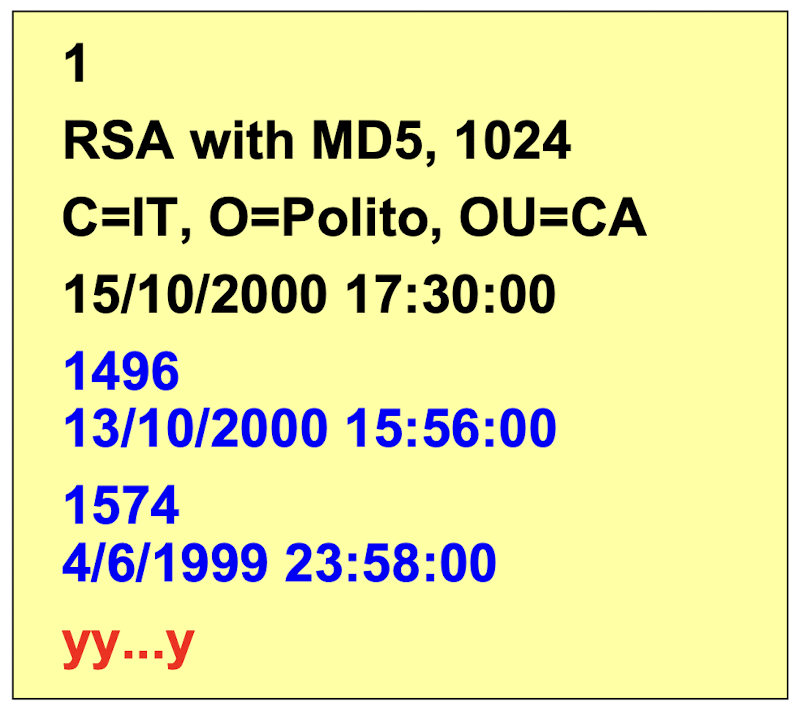
\includegraphics[width=\linewidth]{Images/Cryptography/x509_crl.png}
        \caption{X.509 CRL structure}
    \end{figure}
\end{multicols}

\subsection{Verification of a Signature/Certificate}

\begin{tcolorbox}[colback=blue!10!white, colframe=blue!50!white]
    It is necessary to have an infrastructure for the certification and distribution of public-key certificates, as well as for the dissemination of their respective revocation information.
\end{tcolorbox}

\begin{center}
    \textbf{The Process}
\end{center}
The verifies must:
\begin{enumerate}
    \item Check if the public key of the sender is valid (created within the validity period of the certificate) and the public key certificate was issued by a trusted CA.
    \item Decrypt the digital signature using the public key of the sender ($X$). The decrypted value represents the digest extracted from the signature.
    \item Calculate the hash of the data (message or file) using the same hash function as the signer.
    \item Compare the two digests: If they match, the signature is valid, confirming both the authenticity (the signature belongs to $X$) and the integrity (the data has not been altered).
    \item If the digests do not match, the signature is invalid, indicating either tampering with the data or an incorrect public key.
    \end{enumerate}
\begin{figure}[H]
    \centering
    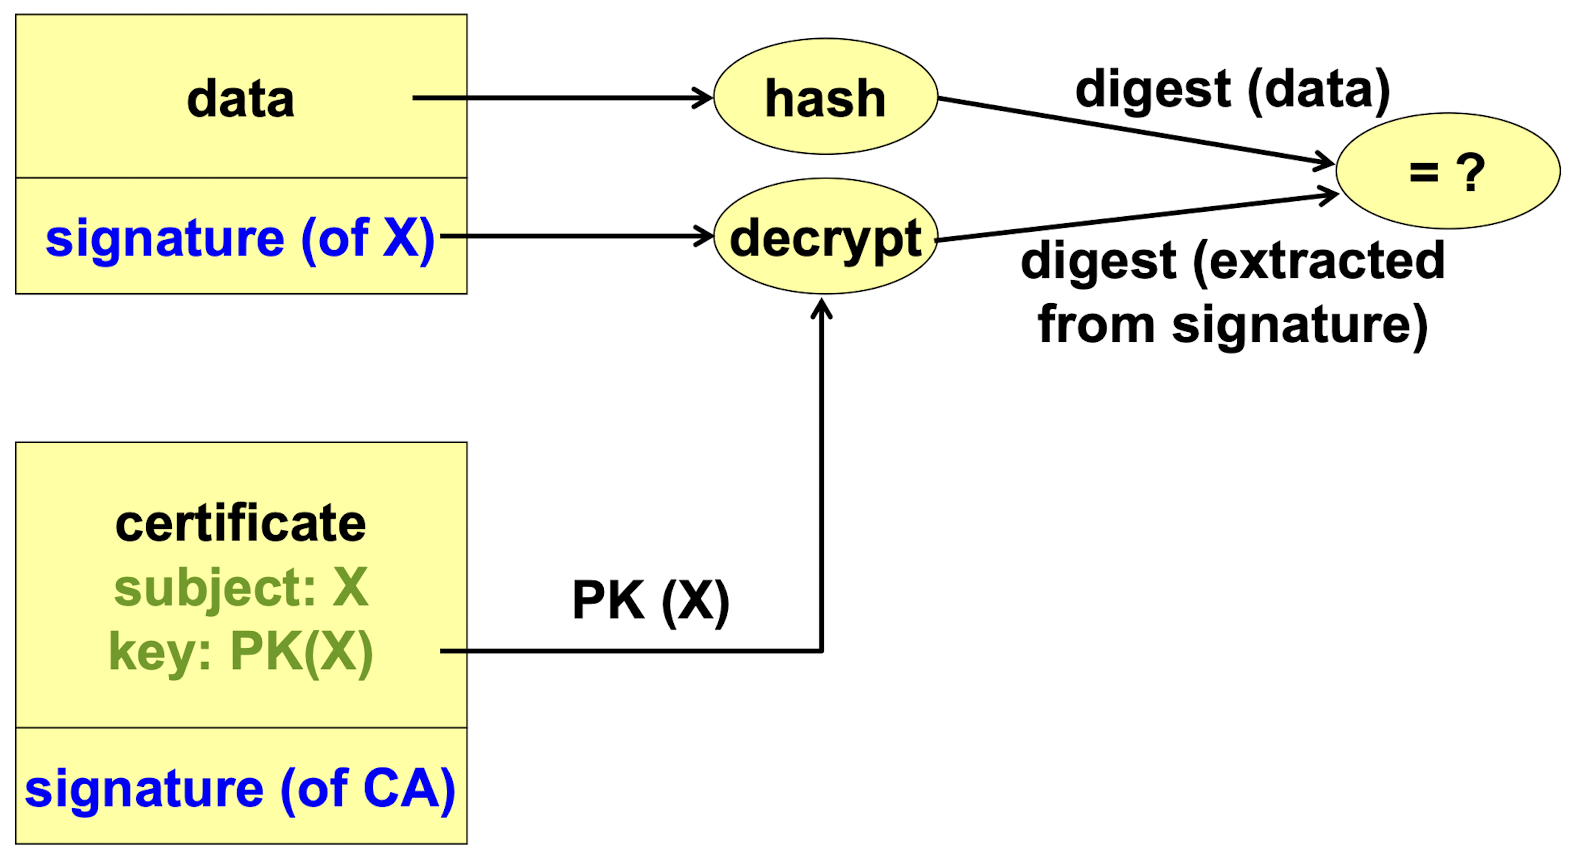
\includegraphics[width=0.5\linewidth]{Images/Cryptography/cert_verif.png}
    \caption{Verification process of a Signature/Certificate}
\end{figure}

\subsection{Certification Hierarchy}
\begin{center}
    (Chain of Trust)
\end{center}
The diagram \ref{fig:cert_hier} illustrates the Certification Hierarchy (also called the Chain of Trust) in a Public Key Infrastructure (PKI).

\hfill

Starting from the top:
\begin{enumerate}
    \item Top-Level Certification Authority (TLCA or Root CA): The highest level of the hierarchy, which issues certificates to intermediate CAs. It is the trusted entity that signs certificates for lower-level Certification Authorities (CAs). 
    \[
        \text{All trust starts here, and this CA is implicitly trusted in the PKI.}
    \]
    \item Intermediate Certification Authority (ICA): An entity that issues certificates to end entities (users, servers, etc.).
    \item Lower-Level (Local) CAs.
\end{enumerate}
\begin{tcolorbox}[colback=red!10!white, colframe=red!70!black, coltitle=white, title=Beware]
    Each CA at any level in the hierarchy signs certificates with its digital signature (ds). The signature is verified by the next higher-level CA in the hierarchy.
\end{tcolorbox}
\begin{figure}[H]
    \centering
    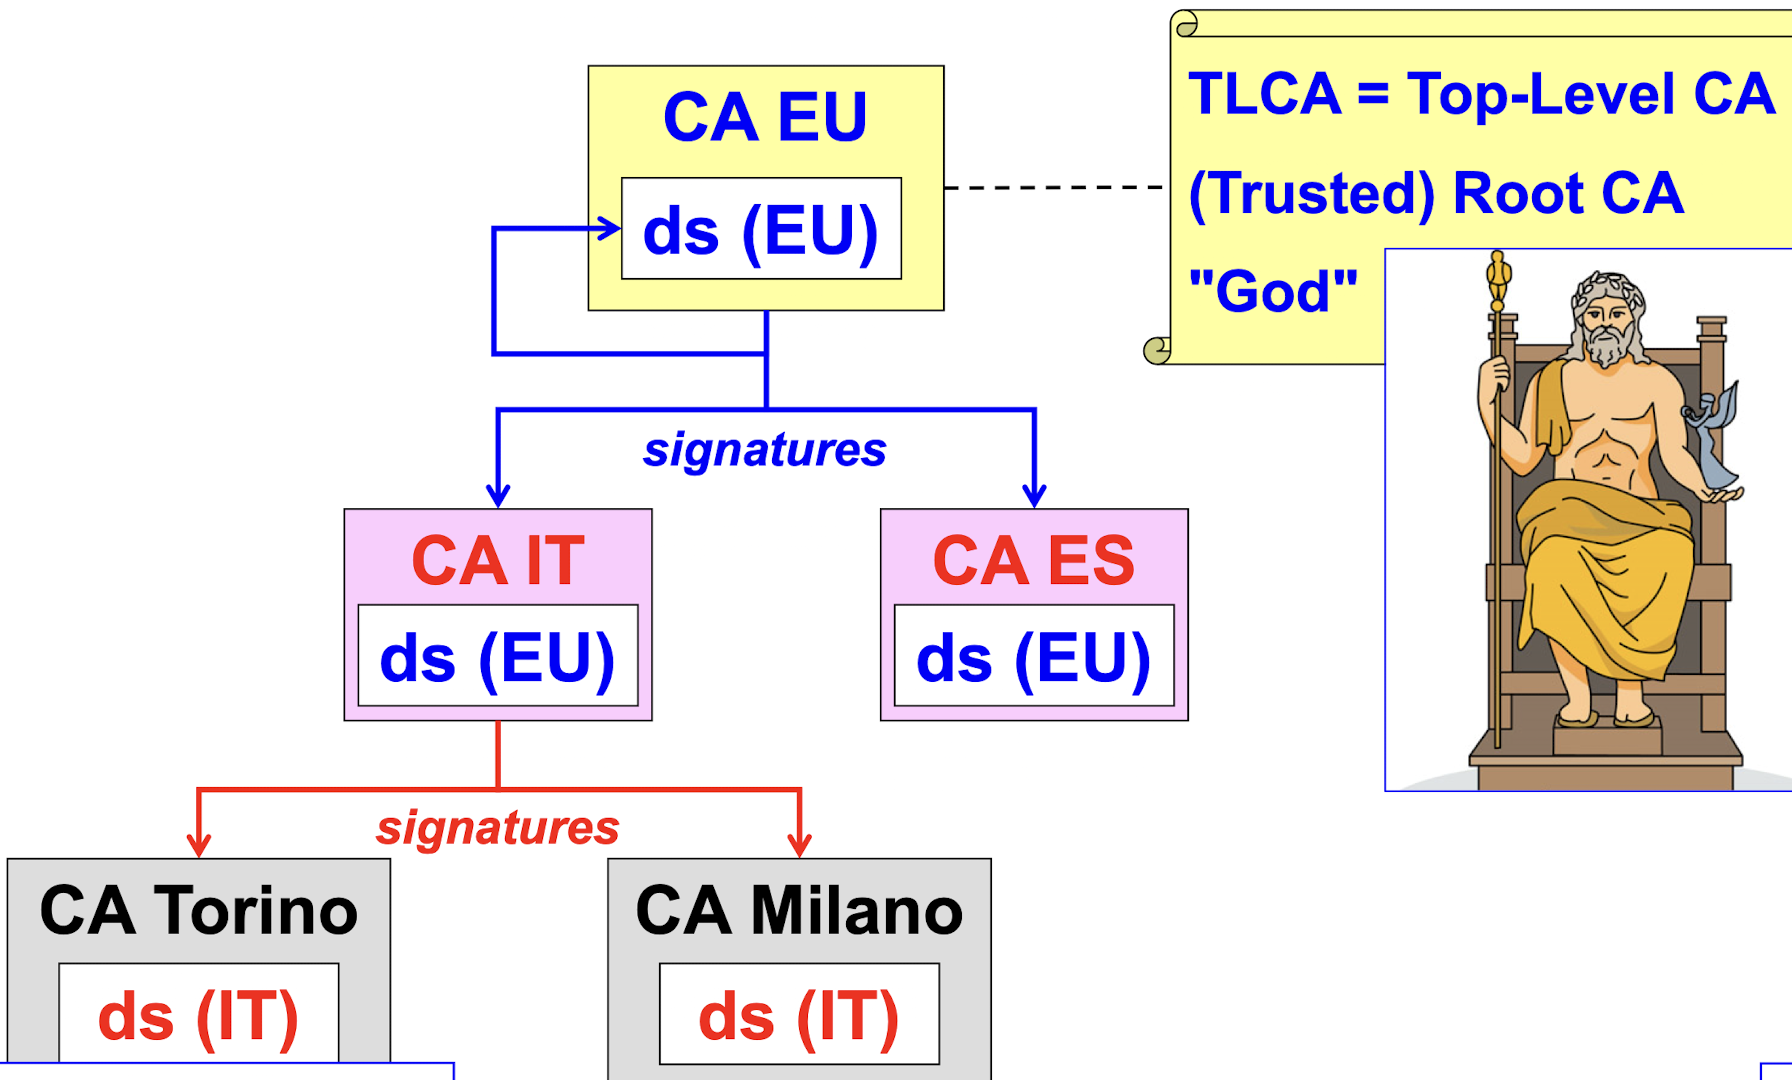
\includegraphics[width=0.5\linewidth]{Images/Cryptography/cert_hier.png}
    \caption{Example of Certification Hierarchy}
    \label{fig:cert_hier}
\end{figure}

\section{Commercial National Security Algorithm Suite}
\begin{center}
    CNSA Suite 2018
\end{center}
Includes the following algorithms:
\begin{itemize}
    \item Symmetric Encryption: AES-256 (Advanced Encryption Standard 256), with mode CTL (low bandwidth) or GCM (high bandwidth).
    \item Hashing: SHA-384 (Secure Hash Algorithm 512 truncated to 384 bits).
    \item Key Agreement: ECDH-384 (Elliptic Curve Diffie-Hellman) and ECMQV (Elliptic Curve Menezes-Qu-Vanstone).
    \item Digital Signature: ECDSA-384 (Elliptic Curve Digital Signature Algorithm).
    \item Elliptic Curve (EC): Curve P-384.
    \end{itemize}
    
    For legacy systems:
    \begin{itemize}
    \item Key Agreement: DH-3072 (Diffie-Hellman).
    \item Key Exchange and Digital Signature: RSA-3072 (Rivest-Shamir-Adleman).
    \end{itemize}
    
    \vspace{1cm}
    
    \begin{center}
    CNSA Suite 2022
    \end{center}
    
    Includes the following algorithms:
    \begin{itemize}
    \item Symmetric Encryption: AES-256 (Advanced Encryption Standard 256), with mode CTL (low bandwidth) or GCM (high bandwidth).
    \item Hashing: SHA-384 or SHA-512.
    \item Key Agreement: CRYSTALS-Kyber with level V parameters.
    \item Digital Signature: CRYSTALS-Dilithium with level V parameters.
    \item Digital Signature for Firmware and Software:
    \begin{itemize}
    \item All NIST SP 800-208 algorithms (LMS, XMSS).
    \item Suggested: LMS SHA-256/192.
    \end{itemize}
    \end{itemize}


\bibliographystyle{unsrt}
\bibliograph